\documentclass{article}

\usepackage{arxiv}
%\usepackage[n, 
%% or lambda advantage , operators , sets,
%adversary , landau , probability , notions ,
%logic ,ff, mm,
%primitives , events , complexity , oracles , asymptotics , keys]{cryptocode}
\usepackage[utf8]{inputenc}
\usepackage{bbm}
\usepackage{xcolor}
\usepackage[utf8]{inputenc} % allow utf-8 input
\usepackage[T1]{fontenc}    % use 8-bit T1 fonts
\usepackage{hyperref}       % hyperlinks
\usepackage{url}            % simple URL typesetting
\usepackage{booktabs}       % professional-quality tables
\usepackage{amsfonts}       % blackboard math symbols
\usepackage{nicefrac}       % compact symbols for 1/2, etc.
\usepackage{microtype}      % microtypography
\usepackage{amsthm}
\usepackage{tikz}
\usepackage{tabularx}
\usepackage[most]{tcolorbox}
\usepackage{cleveref}       % smart cross-referencing
\usepackage{lipsum}         % Can be removed after putting your text content
\usepackage{graphicx}
\usepackage{algorithm}
\usepackage{stmaryrd} % llbracket stuff
%\usepackage{hyperref}
\usepackage[square,sort,comma,numbers]{natbib}
\usepackage{doi}
\graphicspath{ {assets/} }
\usepackage{bbding}
\usepackage[colorinlistoftodos,prependcaption]{todonotes}
\usepackage[n, 
% or lambda advantage , operators , sets,
adversary , landau , probability , notions ,
logic ,ff, mm,
primitives , events , complexity , oracles , asymptotics , keys]{cryptocode}

\usepackage{stmaryrd}

% FONT For The paper
\usepackage{sans}
\usepackage[T1]{fontenc}
\renewcommand\familydefault{\sfdefault}
\usepackage{setspace}
\onehalfspacing


\definecolor{amber}{rgb}{1.0, 0.49, 0.0}
\definecolor{cadmiumgreen}{rgb}{0.0, 0.42, 0.24}
\definecolor{darkcyan}{rgb}{0.0, 0.55, 0.55}
\definecolor{darkcoral}{rgb}{0.8, 0.36, 0.27}
\definecolor{azure}{rgb}{0.0, 0.5, 1.0}
\definecolor{bittersweet}{rgb}{1.0, 0.44, 0.37}
\definecolor{razzmatazz}{rgb}{0.89, 0.15, 0.42}

\hypersetup{
  colorlinks,
  citecolor=cadmiumgreen,
  linkcolor=azure,
  urlcolor=azure}
  



\newtheoremstyle{theorem}%
{3pt}% Space above
{3pt}% Space below 
{}% Body font
{}% Indent amount
{\bfseries\color{razzmatazz}}% Theorem head font
{}% Punctuation after theorem head
{.5em}% Space after theorem head
{}% Theorem head spec (can be left empty, meaning ‘normal’)
\theoremstyle{theorem}
\newtheorem{thm}{Theorem}
\newtheorem{lemma}{Lemma}
\newtheorem{claim}{Claim}
\newtheorem{fact}{Fact}
\newtheorem{corollary}{Corollary}

\newtheoremstyle{definition}%
{3pt}% Space above
{3pt}% Space below 
{}% Body font
{}% Indent amount
{\bfseries\color{darkcyan}}% Theorem head font
{}% Punctuation after theorem head
{.5em}% Space after theorem head
{}% Theorem head spec (can be left empty, meaning ‘normal’)
\theoremstyle{definition}
\newtheorem{definition}{Definition}
\newtheorem{goal}{Goal}


\newtheoremstyle{remark}%
{3pt}% Space above
{3pt}% Space below 
{}% Body font
{}% Indent amount
{\bfseries\color{razzmatazz}}% Theorem head font
{}% Punctuation after theorem head
{.5em}% Space after theorem head
{}% Theorem head spec (can be left empty, meaning ‘normal’)
\theoremstyle{remark}
\newtheorem{remark}{Remark}


%\newcommand{\stateclaimsolid}[2]{
%  \par\noindent\tikzstyle{mybox} = [draw=black,fill=yellow!20,
%   thick,rectangle,rounded corners, inner sep=6pt,path picture={\fill ([xshift=-6.15cm]path picture bounding box.north) rectangle (path picture bounding box.south west);}]
%  \begin{tikzpicture}
%   \node [mybox] (box){%
%    \begin{minipage}{#1}{#2}\end{minipage}
%   };
%  \end{tikzpicture}
%}

\newcommand{\stateboxsolid}[1]{
  \par\noindent\tikzstyle{mybox} = [draw=black,fill=white!20,
   thick,rectangle,rounded corners,inner sep=6pt]
  \begin{tikzpicture}
    \node [mybox] (box){%
    \begin{minipage}{0.99\textwidth}{#1}\end{minipage}
   };
  \end{tikzpicture}
}
\newcommand{\statetheoremsolid}[2]{
  \par\noindent\tikzstyle{mybox} = [draw=black,fill=yellow!20,
   thick,rectangle,rounded corners,inner sep=6pt]
  \begin{tikzpicture}
    \node [mybox] (box){%
    \begin{minipage}{#1}{#2}\end{minipage}
   };
  \end{tikzpicture}
}
% TIKZ stuff above

% Typical re-transformations
%\renewcommand{\epsilon}{\varepsilon}
\newcommand{\bit}{\{ 0, 1\}}
\renewcommand{\poly}{\mathsf{poly}}
%\newcommand{\pp}{\mathtt{pp}}
\newcommand{\samples}{\xleftarrow{\$}}
\newcommand{\inputs}{\xleftarrow{\mathsf{input}}}
\newcommand{\outputs}{\xrightarrow{\mathsf{output}}}
\newcommand{\samplesIdd}{\xleftarrow{\mathsf{i.i.d}}}

\newcommand{\AdvA}{\ensuremath{\mathcal{A}}}
\renewcommand{\oracle}{\ensuremath{\mathcal{O}}}

\newcommand{\PermDist}{\mathcal{D}}
\newcommand{\FarPermDist}{\hat{\mathcal{D}}}


\newcounter{protocol}
\newenvironment{protocol}[1]
  {\par\addvspace{\topsep}
   \noindent
   \tabularx{\linewidth}{@{} X @{}}
    \hline
    \refstepcounter{protocol}\textbf{Protocol \theprotocol} #1 \\
    \hline}
  { \\
    \hline
   \endtabularx
   \par\addvspace{\topsep}}

\newcommand{\xmark}{\text{}}


\newcommand{\etal}{\textit{et al.}{ }}
\newcommand{\bin}{\mathtt{Bin}}

\newcommand{\Z}{\mathbb{Z}}
\newcommand{\F}{\mathbb{F}}
\newcommand{\R}{\mathbb{R}}
\newcommand{\G}{\mathbb{G}}
\renewcommand{\pp}{\texttt{pp}}
\newcommand{\noisen}{\eta}
\newcommand{\Mechanism}{\mathtt{M}}

\renewcommand{\OR}{\mathsf{OR}}
\newcommand{\OrProtocol}{\Pi_\OR}
\newcommand{\BitLang}{\mathsf{L}_{\mathsf{Bit}}}
\newcommand{\Setup}{\mathtt{Setup}}
\newcommand{\Morra}{\mathtt{morra}}
\newcommand{\Output}{\mathtt{out}}
\newcommand{\share}[1]{\llbracket #1 \rrbracket}
\renewcommand{\gets}{\xleftarrow{\texttt{Input}}}
%\newcommand{\SecretShare}[2]{\Big( [#1]_{1}, \dots, [#1]_{#2}\Big)}

% Commitment stuff
\newcommand{\RandomnessSpace}{\mathsf{Rand}}
\newcommand{\MessageSpace}{\mathsf{Msg}}


\DeclareMathOperator{\Com}{Com}
\renewcommand{\bin}{\mathsf{Bin}}
%text symbols
\newcommand{\SecurityParam}{\kappa}
\newcommand{\Naturals}{\mathbb{N}}
\newcommand{\Normal}{\mathcal{N}}
\newcommand{\Integers}{\mathbb{Z}}
\newcommand{\Reals}{\mathbb{R}}
\newcommand{\Identity}{\mathit{I}}
\newcommand{\Exp}{\mathsf{exp}}
\renewcommand{\exp}{\Exp}
\newcommand{\Eps}{\varepsilon}
\newcommand{\EpsDelta}{(\Eps, \delta)}

%functions
\newcommand{\FuncDomain}{\mathcal{X}}
\newcommand{\FuncRange}{\mathcal{Y}}
\newcommand{\FuncFamily}{\mathcal{Q}}
\DeclareMathOperator*{\argmax}{arg\,max}
\DeclareMathOperator*{\argmin}{arg\,min}

%graphs
\newcommand{\Vertices}{\mathcal{V}}
\newcommand{\Edges}{\mathcal{E}}
\newcommand{\Adjacency}{\mathtt{Adj}}
\newcommand{\Incidence}{\mathtt{Inc}}
\newcommand{\hamming}[1]{d_\mathtt{Ham} #1}

%distributions
\newcommand{\Dist}{\mathcal{D}}
\newcommand{\Support}{\mathsf{Support}}

\newcommand{\SuppSize}{\mathsf{n}}
\newcommand{\DomainDist}{\Omega_{\SuppSize}}
\newcommand{\DomainDistJoint}{\Omega_{\mathsf{n_1} \times \mathsf{n_2}}}
\newcommand{\DomainDistJointSame}{\Omega_{\mathsf{n} \times \mathsf{n}}}
\newcommand{\DistSet}{\Delta(\DomainDist)}
\newcommand{\DistSetJoint}{\Delta(\DomainDistJoint)}
\newcommand{\DistSetJointSame}{\Delta(\DomainDistJointSame)}
\newcommand\TotalVar[2]{d_{\textsf{TV}}(#1,#2)}
\newcommand{\Negl}{\mu}
\newcommand{\AvgMinEntropy}{\tilde{H}_\infty}


%distribution testing
\newcommand{\DIP}{\mathsf{DIP}}
\newcommand{\EZKDIP}{\mathsf{EZKDIP}}
\newcommand{\ZKDIP}{\mathsf{ZKDIP}}
\newcommand{\SZKDIP}{\mathsf{SZKDIP}}
\newcommand{\HVCZK}{\mathsf{HVCZK}}
\newcommand{\HVCZKD}{\mathsf{HVCZK-D}}
\newcommand{\out}{\mathsf{out}}
\newcommand{\Tester}{\mathsf{T}}
\newcommand{\Verifier}{\mathsf{V}}
\newcommand{\Prover}{\mathsf{P}}
\newcommand{\Sender}{\mathsf{S}}
\newcommand{\Receiver}{\mathsf{R}}
\newcommand{\ChSender}{\mathsf{\hat{S}}}
\newcommand{\ChReceiver}{\mathsf{\hat{R}}}
\newcommand{\ChVerifier}{\mathsf{\hat{V}}}
\newcommand{\ChProver}{\mathsf{\widetilde{P}}}
\newcommand{\OptProver}{\mathsf{P}^*}
\newcommand{\Simulator}{\mathsf{Sim}}
\newcommand{\AuxInput}{z}
\newcommand{\View}{\mathrm{view}}
\newcommand{\Prop}{\Pi}
\newcommand{\PropJoint}{\Pi_{\mathsf{n_1} \times \mathsf{n_2}}}
\newcommand{\PropJointSame}{\Pi_{\mathsf{n} \times \mathsf{n}}}
\newcommand{\Proximity}{\delta}
\newcommand{\Accept}{\textsf{accept}}
\newcommand{\Reject}{\textsf{reject}}
\newcommand{\interacton}[2]{ \left(#1, #2 \right)}
\newcommand{\VerifierLocalRand}{\vec{\rho}}
\newcommand{\TV}[1]{d_\mathtt{TV} #1}
\newcommand{\EM}[1]{d_\mathtt{EM} #1}
\newcommand{\statInd}{\stackrel{s}{\equiv}}
\newcommand{\compInd}{\stackrel{c}{\equiv}}


%permuatations
\newcommand{\PermProp}{\Prop^\mathsf{BIJECT}_n}
\newcommand{\PermSize}{n}
\newcommand{\Perm}{f}
\newcommand{\Bad}{\mathsf{Bad}}
\newcommand{\Good}{\mathsf{Good}}


%permutation protocol
\newcommand{\NumSamples}{k}
\newcommand{\NumRounds}{T}
\newcommand{\RandRound}{t}
\newcommand{\RoundInd}{\mathsf{round}}
\newcommand{\PermSamplePoint}{x}
\newcommand{\PermChallengePoint}{y}
\newcommand{\Challenge}{\mathsf{CHALLENGE}}
\newcommand{\NotPerm}{\hat{f}}
\newcommand{\PermProver}{\mathsf{P}_{\text{perm}}}
\newcommand{\PermVerifier}{\mathsf{V}_{\text{perm}}}

\newcommand{\Cheat}{\mathsf{Cheat}}
\newcommand{\True}{\mathsf{TRUE}}
\newcommand{\No}{\mathsf{No}}
\newcommand{\Yes}{\mathsf{Yes}}
\newcommand{\False}{\mathsf{FALSE}}
\newcommand{\calR}{\mathcal{R}}

% computational ZK
\newcommand{\com}{\mathtt{com}}

%mathsf
\newcommand{\sfA}{\mathsf{A}}


%complexity classes
\newcommand{\eIPP}{\ensuremath{\Proximity\mathsf{-IPP}}}

\newcommand{\sbline}{\\[.5\normalbaselineskip]}% small blank line
\newcommand\inner[2]{\langle #1, #2 \rangle}
\newcommand\Biginner[2]{\Big\langle #1, #2 \Big\rangle}
\newcommand{\boocube}{\{0, 1\}^n}
\newcommand{\boodist}{\Delta(\boocube,\boocube)}

%operators
\newcommand{\pST}{\; \middle| \;}

%formatting
\newcommand{\DoQuote}[1]{``#1''}
\newcommand{\defemph}[1]{\textbf{\emph{#1}}}


%notes
\newcommand{\ariInline}[1]{\todo[backgroundcolor=azure!15, bordercolor=azure, textcolor=black, inline]{#1 - Ari}}
\newcommand{\ari}[1]{\todo[backgroundcolor=azure!15, bordercolor=azure, textcolor=black]{#1 - Ari}}

\newcommand{\NR}[1]{\todo[backgroundcolor=bittersweet!15, bordercolor=bittersweet, textcolor=black, inline]{#1 - Ninad}}

\newcommand{\highlight}[1]{\color{razzmatazz}\textit{#1 }\color{black}}
%\newtheorem{definition}{Definition}[section]
%\newtheorem{remark}[definition]{Remark}
%\newtheorem{theorem}[definition]{Theorem}
%\newtheorem{lemma}[definition]{Lemma}
%\newtheorem{corollary}[definition]{Corollary}
%\newtheorem{prop}[definition]{Proposition}



\title{Interactive Proofs For Differentially Privacy\thanks{A Preliminary version of this work is set to appear at The ACM Conference on Computer and Communications Security (CCS), 2023}}

% Here you can change the date presented in the paper title
%\date{September 9, 1985}
% Or remove it
%\date{}

\author{\href{https://abiswas3.github.io}{Ari Biswas}\\
	University Of Warwick\\
	\texttt{aribiswas3@gmail.com} \\
	%% examples of more authors
	\AND
	\href{https://warwick.ac.uk/fac/sci/dcs/people/graham_cormode/}{Graham Cormode}\\
	University Of Warwick/Meta AI \\
	\texttt{gcormode@meta.com}
	%% \And
	%% Coauthor \\
	%% Affiliation \\
	%% Address \\
	%% \texttt{email} \\
	%% \And
	%% Coauthor \\
	%% Affiliation \\
	%% Address \\
	%% \texttt{email} \\
}

% Uncomment to override  the `A preprint' in the header
\renewcommand{\headeright}{Appear at CCS 2023}
\renewcommand{\undertitle}{}
\renewcommand{\shorttitle}{\textit{arXiv} Template}

%%% Add PDF metadata to help others organize their library
%%% Once the PDF is generated, you can check the metadata with
%%% $ pdfinfo template.pdf
%\hypersetup{
%pdftitle={Meh},
%pdfsubject={q-bio.NC, q-bio.QM},
%pdfauthor={David S.~Hippocampus, Elias D.~Striatum},
%pdfkeywords={First keyword, Second keyword, More},
%}

\begin{document}
\maketitle

\begin{abstract}
  Differential Privacy (DP) is often presented as a strong
  privacy-enhancing technology with broad applicability and advocated
  as a de-facto standard for releasing aggregate statistics on
  sensitive data.  However, in many embodiments, DP introduces a new
  attack surface: a malicious entity entrusted with releasing
  statistics could manipulate the results and use the randomness of DP
  as a convenient smokescreen to mask its nefariousness.  Since
  revealing the random noise would obviate the purpose of introducing
  it, the miscreant may have a perfect alibi.  To close this loophole,
  we introduce the idea of \textit{Interactive Proofs For Differential
    Privacy}, which requires the publishing entity to output a zero
  knowledge proof that convinces an efficient verifier that the output
  is both DP and reliable.  Such a definition might seem unachievable,
  as a verifier must validate that DP randomness was generated
  faithfully without learning anything about the randomness itself.
  We resolve this paradox by carefully mixing private and public
  randomness to compute verifiable DP counting queries with
  theoretical guarantees and show that it is also practical for
  real-world deployment.  We also demonstrate that computational
  assumptions are necessary by showing a separation between
  information-theoretic DP and computational DP under our definition
  of verifiability.
\end{abstract}


% keywords can be removed
%\keywords{First keyword \and Second keyword \and More}

\section{Introduction}
\label{sec:introduction}

We are living in an age of delegation, where the bulk of our digital
data is held and processed by others in an opaque fashion.  Our
interactions are collated by digital applications that continually
send our personal information to the ``cloud''.  Servers in the cloud,
typically owned by large monolithic organizations, such as Google, AWS
or Microsoft, then perform computations on our private data to publish
aggregate statistics for social utility.  For example, we send our GPS
coordinates to services like Strava and Google which, in exchange, use
this information to recommend low-traffic cycling
routes~\cite{raturi2021impact}.  Similarly, we let entertainment
companies like Netflix, YouTube, TikTok and Hulu know our personal
preferences so that they can better recommend content for us to
consume~\cite{bell2007lessons}.  National census bureaus collect
personal information to publish aggregate statistics about the
population, and consider doing so a moral duty to ensure transparency
in the government's policies~\cite{boyd2022differential}.

However, it is often the case that published aggregate statistics leak
information about the activity of individuals.  For example, Garfinkel
\etal and Kasiviswanathan \etal describe practical reconstruction
attacks that can be used to infer an individual's private data from
aggregate population statistics ~\cite{garfinkel2019understanding,
  kasiviswanathan2013power}.  Boyd \etal show that published census
data has been used to discriminate against groups in society based on
race ~\cite{boyd2022differential}.  Hence the information that is
released, and how it is computed, requires careful scrutiny.
%In this such cases, the privacy leakage is a property of the functionality being computed, and not the protocol used to compute it. 

In response to these concerns, the privacy and security community have
sought to apply various privacy enhancing technologies to protect the
privacy of individuals contributing to data releases.  Most relevant
to this discussion is Differential Privacy (DP) and its
generalizations, which require computations to be randomized, in order
to offer the (informally stated) promise that users will not be
adversely affected by allowing their data to be used.  Typically, this
is achieved by adding carefully calibrated random noise to the output,
at the expense of reducing the accuracy of the computation.
Differential privacy is most commonly studied in the \textit{trusted
  curator} model, where a single entity receives all the sensitive
data, and is entrusted to execute the algorithm to apply the random
noise.  Variations that modify the trust and computational model
include local privacy \cite{warner1965randomized}, shuffle privacy
\cite{balle2019privacy, champion2019securely}, computational
differential privacy ~\cite{mironov2009computational} and multi-party
differential privacy \cite{mcgregor2010limits}.

A consistent theme across all existing work is to view DP simply as a
privacy-preserving mechanism.  In this paper, we shift the focus and
view differential privacy through an adversarial lens: \highlight{what if
  the entity responsible for releasing aggregate DP statistics seeks to abuse 
  the protocol and pick noise chosen to distort the statistics, using 
  differential privacy as an attack vector?}

That is, a malicious entity may tamper with the computation in order
to publish biased statistics, and claim this reflects the true
outcome; any discrepancies may be dismissed as artifacts of random
noise.  Consider a counting query DP protocol to determine the winner
of a plurality election, where the users vote for 1 out of $M$
candidates (say, which topping people prefer on their pizza).  A
corrupted aggregator might not be interested in any particular user's
vote but in biasing the aggregate output of the protocol instead.
Thus, if that server has auxiliary information about the preferences
of a subset of users, they might tamper with the protocol to exclude
those honest voters from the election or tamper with the protocol to
bias the results of the election (say, to pineapple) and blame any
discrepancies in the result on random noise introduced by DP.  Note
that some loss in accuracy for privacy is unavoidable.  By definition,
DP requires the output be perturbed by private randomness.  Often,
outputting such random statistics creates tensions between publishing
entity and the downstream consumer.  In 2021, the State Of Alabama
filed a lawsuit claiming that the use of DP on census data was
illegal~\cite{courtCase}, citing the inaccuracies introduced by DP.
Thus, to ensure public trust in DP, it is critical to verify that any
loss in utility can be attributed solely to unavoidable DP randomness.

To that effect, we formally introduce the idea of
\textit{Interactive Proofs For 
  Differential Privacy} in both the trusted curator \footnote{When we say trusted curator, we imply that there is a single server that can view client inputs in plaintext. However, this server could still be corrupted and therefore, it must prove that the final released output was computed as prescribed the DP protocol. Of course in the single server setting we cannot protect client privacy. The focus is on ensuring the output is reliable}  setting and the multi-party setting in presence of active adversaries
  \footnote{By active adversaries, we mean participants that may deviate from protocol specifications arbitrarily. In the MPC setting we can guarantee both privacy of client inputs and reliability of output.}. Our contributions are as
follows:

\begin{enumerate}

\item{We formally introduce definitions for
    \textit{Interactive Proofs For Differential Privacy} in
    both the trusted curator and client-server multiparty setting
    \cite{baum2014publicly}. Informally, the entity responsible for
    releasing DP statistics must also output a
    zero knowledge proof to verify that the statistic was computed
    correctly with respect to committed client inputs and the private randomness generated faithfully. Such a
    proof reveals no additional information and still enforces that
    user privacy is protected via DP but ensures that the curator
    cannot use DP randomness maliciously.}

\item{We show concrete instantiations of verifiable DP by computing DP
    counting queries (histograms) in the trusted curator and
    client-server multiparty settings. In the trusted curator
    setting, there is a single aggregating server that sees client
    data in plaintext and is responsible for outputting a DP histogram
    and a proof that the DP noise was generated faithfully. In the
    client-server MPC setting, clients secret share the inputs and
    send them to $K \geq 2$ servers, who then participate in an MPC
    protocol to output DP histograms. The protocol itself is secure in
    that not even the participating servers are able to learn any new
    information beyond the output nor are they able to tamper with the
    protocol.}
    
\item{We conduct experiments to show that our protocols with formal
    theoretical guarantees are also practical.  Additionally, we
    describe how our protocol $\Pi_\bin$, for verifiable DP counting,
    can be combined with existing (non-verifiable) DP-MPC protocols,
    such as PRIO \cite{corrigan-gibbs_prio_2017} and Poplar
    \cite{boneh_lightweight_2022}, to enforce verifiability.}
	

\item{We demonstrate that information-theoretic verifiable DP is
    impossible. Specifically, if both the prover and verifier are
    computationally unbounded, then statistical zero knowledge
    and unconditional soundness cannot hold simultaneously. Thus we could either
    prevent an all-powerful curator from manipulating DP protocols or
    an all-powerful verifier from being able to distinguish between
    neighbouring datasets from the output, but not both.  This result
    is related to an open problem (Open Problem 10.6) of
    Vadhan~\cite{vadhan2017complexity}, which asks \textit{``Is there
      a computational task solvable by a single curator with
      computational differential privacy but is impossible to achieve
      with information-theoretic differential privacy?''}.  In Section
    \ref{sec:separation} we relate our result to efforts at resolving
    this question.}

\end{enumerate}


\section{Preliminaries}
\label{sec:prelims}

\paragraph{General Notation}

We write $x \samples U$ to denote that $x$ was uniformly sampled from a set $U$. We write $A \gets (a,b,c)$ to denote that an algorithm $A$ receives $a,b$ and $c$ as inputs.
We denote vectors with an arrow on top as in $\vec{x} \in \Z_q^M$, where $M$ represents the number of coordinates
in the vector and $\Z_q$ represents a prime order finite field of integers of size $q$. 
We write $\vec{a} + \vec{b}$ to mean coordinate-wise vector addition $a + b \mod q$, where $a$ and $b$ correspond to values at the same position of $\vec{a}$ and
$\vec{b}$.  
Similarly, when we write $\vec{a} \times \vec{b}$, we refer to the coordinate-wise Hadamard product between the two vectors.

\paragraph{Public Parameters}

\paragraph{MPC setting}

\paragraph{Privacy and Security Background}
\label{sec:background}

%Negligible
\begin{definition}[Negligible Functions]
A function $\Negl: \Naturals \rightarrow \Reals$	is negligible iff $\forall c \in \Naturals$, there $\exists n_c \in \Naturals$, such that $\forall n > n_c$, $\mu(n) \leq n^{-c}$.
\end{definition}

% Stat Ind
\begin{definition}[Statistical Distinguishablity] We say two probability ensembles $\{ X_n\}_{n \in \Naturals }$ and  $\{ Y_n\}_{n \in \Naturals}$ are statistically indistinguishable if there exists a negligible function $\Negl$ such that, for all sufficiently large $n$'s it holds that 

\begin{equation*}
	 \TV{(X_n, Y_n)} \leq \Negl(n)
\end{equation*} 

We denote two statistically indistinguishable distributions as $\{ X_n\}_{n \in \Naturals} \statInd \{
  Y_n\}_{n \in \Naturals}$. If we have $\Negl(n) = 0$, we say the two distributions are perfectly indistinguishable and we denote it as $\{ X_n\}_{n \in \Naturals} \equiv \{
  Y_n\}_{n \in \Naturals}$.
	
\end{definition}

\begin{definition}[Computational Indistinguishability]
  \label{defn:indisitinguish} Let $\{ X_n\}_{n \in \Naturals }$ and $\{ Y_n\}_{n \in \Naturals }$ be a pair of ensembles where $X_n$ and $Y_n$ are probability distributions over $\bit^{\poly(n)}$. 
We say that $\{ X_n\}_{n \in N }$ and $\{ Y_n\}_{n \in \Naturals }$
  are computationally indistinguishable if for all non-uniform PPT Turing machines $D$ (``distinguishers''), there exists a negligible function $\Negl$, such that for every $n \in \Naturals$

\begin{equation*}
    \Big| \Pr[D(X_n) = 1] - \Pr[D(Y_n) = 1] \Big| \leq \Negl(n) 
\end{equation*}
  
We denote computational indistinguishability as $\{ X_n\}_{n \in \Naturals} \compInd \{
  Y_n\}_{n \in \Naturals}$.
   
\end{definition}

%\paragraph{Commitments}Commitments are used in our schemes to ensure that participants cannot change their response during the protocol.

\begin{definition}[Non Interactive Commitment Schemes] \label{def:commitments}Let $\SecurityParam \in \Naturals$ be the security
  parameter. 
  A non-interactive commitment scheme consists of a pair of
  probabilistic polynomial time algorithms (\texttt{Setup, Com}). 
  The setup algorithm $\pp \samples \texttt{Setup}(1^\SecurityParam)$ generates
  public parameters $\pp$ for a given security parameter $\SecurityParam$. 
  Given sets $\texttt{M}_{\pp}$ (message space) and $\texttt{R}_{\pp}$ (random space), the commitment algorithm
  $\texttt{Com}_{\pp}$ defines a function
  $\texttt{M}_{\pp} \times \texttt{R}_{\pp} \rightarrow
  \texttt{C}_{\pp}$ that maps a message from the message space to the commitment space
  $\texttt{C}_{\pp}$ using the random space. For a message
  $x \in \texttt{M}_\pp$, the algorithm samples
  $r_x \samples \texttt{R}_\pp$ and computes
  $c_x = \texttt{Com}_{\pp}(x, r_x)$. When the context is clear, will
  drop the subscript and write $\texttt{Com}_\pp $ as $\texttt{Com}$.
\end{definition}

\begin{definition}[Homomorphic Commitments]
\label{defn:hom_coms}
A homomorphic commitment scheme is a non-interactive commitment scheme
such that $\texttt{M}_\pp$ and $ \texttt{R}_\pp$ are fields (with
$(+, \times)$) and $\texttt{C}_\pp$ is an abelian group with the
$\otimes$ operator, such
that for all $x_1, x_2 \in \texttt{M}_\pp$ and
$r_1, r_2 \in \texttt{R}_\pp$ we have
%
\begin{equation}
\label{eq:hom_coms}
\texttt{Com}(x_1, r_1) \otimes \texttt{Com}(x_2, r_2) = \texttt{Com}(x_1 + x_2, r_1 + r_2)
\end{equation}
\end{definition}


% \textbf{Vector Notation For Commitments}: We define a vector commitment for  a vector $\vec{x} = (x_1, \dots, x_M)$ as the coordinate wise commitment of each coordinate of $\vec{x}$ using a random vector $(r_{1}, \dots, r_{M}) = \vec{r} \samples \texttt{R}_\pp^M$
% %
% \begin{equation}
% \Com(\vec{x}, \vec{r}) =  \vec{c_x}
% \end{equation}
% When we write $\vec{c}_x \times \vec{c}_y$, we mean the Hadamard product over $\G_q^M$. 

Throughout this paper, when we use a commitment scheme, we mean a non-interactive homomorphic commitment scheme  with the following properties (stated informally here, but formalised in the Appendix \ref{app:sec_defns}): 

\begin{enumerate}
    \item{\textbf{Hiding:}  A commitment $c_x$ reveals no information about $x$ and $r_x$ to a computationally bounded adversary (Definition~\ref{defn:hiding_com}).}

    \item{\textbf{Binding:} Given a commitment $c_x$ to $x$ using $r_x$, there is no efficient algorithm that can find $x^\prime$ and $r_{x^\prime}$ such that $\Com(x^\prime, r_{x^\prime}) = c_x = \Com(x, r_{x})$ (Definition~\ref{defn:binding_com}).}

    \item{\textbf{Zero Knowledge OR Opening:} Given $c_x$, the committing party can prove to a polynomial time verifier that $c_x$ is a commitment to either 1 or 0 without revealing which one it is. We denote such a proof as $\Pi_{\texttt{OR}}$ and say it securely computes the oracle $\oracle_{\texttt{OR}}$, which returns true if $c_x \in L_{\texttt{Bit}}$ 
    \begin{equation}
        L_{\texttt{Bit}} = \{c_x: x \in \bit \land  r_x \in \Z_q \land c_x = \Com(x, r_x) \}
    \end{equation}
    See Appendix \ref{app:sigma_open} for a concrete construction of the $\Sigma$-OR proof using Pedersen Commitment schemes from~\cite{damgaard2000efficient}.
    }
\end{enumerate}

In all our experiments and security proofs, we use Pedersen Commitments (PC), though one could replace PC with ~\cite{weng2021wolverine, dittmer2020line, baum2021mathsf}, and still satisfy all the above properties.

\subsection{Differential Privacy As Distribution Testing}

\statetheoremsolid{0.95\textwidth}{
\begin{definition}[Information Theoretic Approximate DP]
\label{def:dp_approx_definition}
Fix $\SecurityParam \in \Naturals$ as the security parameter. Let $n = \poly(\SecurityParam)$ and  $\Eps \geq 0$ and $\Proximity \leq \Negl(n)$ for some negligible function $\Negl$. Let $\FuncFamily  = \{f: \FuncDomain^n \rightarrow \FuncRange \}$ denote a family of functions whose output we wish to make differentially private. Further, assume that the L1 norm is well defined on $\FuncDomain$ and $\FuncRange$. Define a mechanism $\Mechanism: \FuncDomain^n \times \FuncFamily \rightarrow \oracle_{\Delta(\FuncRange)}$ that takes as input $n$ client inputs $X=(x_1, \dots, x_n)$ and a function $f \in \FuncFamily$ and constructs a distribution $\Mechanism(X, f) \in \Delta(\FuncRange)$. It then outputs an oracle $\oracle_{\Mechanism(X,f)}$ that provides sample access to $\Mechanism(X,f)$. $\Mechanism$ satisfies $\Eps$ differential privacy if for \highlight{every} two neighboring datasets $X \sim X^{\prime}$ such that $||X - X^{\prime} ||_1 = 1$ and  for \highlight{every} query $f \in \FuncFamily$ we have \highlight{for all} $T \subseteq \FuncRange$
%
\begin{align}
\label{eq:approx_dp}
    \Pr_{Y \samples M(X, f)}{[ Y \in T]} &\leq e^{\epsilon}\Pr_{Y \samples M(X', f)}{[Y \in T]} + \Proximity
\end{align}
\end{definition}
}


%
%% Information Theoretic DP
%\begin{definition}[Information Theoretic DP~\cite{vadhan2017complexity}]
%\label{def:dp_definitions}
%Fix $n \in \Naturals, \epsilon \geq 0$ and $\delta \leq n^{-\omega(1)}$. Let $\FuncDomain$ and $\FuncRange$ denote metric spaces where the L1 norm $||\cdot ||_1$ is well defined. An algorithm $\Mechanism: \FuncDomain^n \times \FuncFamily \rightarrow \FuncRange$ satisfies $(\epsilon, \delta)$ differential privacy if for every two neighboring datasets $X \sim X^{\prime}$ s.t. $||X - X^{\prime} ||_1 = 1$ and  for every query $Q \in \FuncFamily$ we have for all $T \subseteq \FuncRange$
%%
%\begin{align}
%\label{eq:dp}
%    \Pr_{Y \samples \Mechanism(X, Q)}[Y \in T] &\leq e^{\epsilon}\Pr_{Y \samples \Mechanism(X', Q)}[Y \in T] + \delta
%\end{align}
%\end{definition}

%A direct corollary of the above definition is that, given $M_Q(X)$ and $M_Q(X^\prime)$, with probability $1- \delta$ even an unbounded Turing Machine (TM) $D$ is unable to distinguish between the outputs up to statistical distance $\epsilon$. 


%\paragraph{Computational Differential Privacy (IND-CDP)}
\statetheoremsolid{0.95\textwidth}{
\begin{definition}[IND-CDP~\cite{mironov2009computational}]
\label{def:comp_dp_definitions} 
Fix $\SecurityParam \in \Naturals$ and $n = \poly(\SecurityParam)$. Let $\epsilon \geq 0$ and $\delta(\SecurityParam) \leq \SecurityParam^{-\omega(1)}$ be a negligible function in $\SecurityParam$, and let $\Mechanism = \{ \Mechanism_\SecurityParam : \FuncDomain_\SecurityParam^n \times \FuncFamily \rightarrow  \oracle_{\Delta(\FuncRange_\SecurityParam)} \}_{\SecurityParam \in \Naturals}$ be a family of randomised algorithms, where $\mathcal{X}_\SecurityParam$ and $\mathcal{Y}_\SecurityParam$ can be represented by $\texttt{poly}(\SecurityParam)$-bit strings. 
We say that $\Mechanism$ is \textit{computationally $\epsilon$-differentially private} if for every non-uniform PPT TM's (``distinguisher'') $D$, for every query $f \in \FuncFamily$, and every neighbouring dataset $X \sim X^\prime \in \mathcal{X}_\SecurityParam^n$, for any $T \subseteq \FuncRange_\SecurityParam$ we have 

\begin{equation}    
\Pr_{Y \samples \Mechanism_\SecurityParam(X, Q)}\Big[ D(Y \in T) = 1\Big] \leq e^{\epsilon}\Pr_{Y \samples \Mechanism_\SecurityParam(X^\prime, Q)}\Big[ D(Y \in T) = 1\Big] + \delta(\SecurityParam)
\end{equation}

\end{definition}
}

%\paragraph{DP-Error}

\begin{definition}[DP-Error] Let $\Mechanism: \FuncDomain^n \times \FuncFamily \rightarrow \FuncRange$ be a $\EpsDelta$-DP mechanism for query family $\FuncFamily$ where the $L_1$ norm is well-defined on $\FuncRange$. 
For any $n\in \Naturals$, $X \in \mathcal{X}^n$, we define the expected error of the mechanism $\Mechanism$ relative to $Q$ as 
%
\begin{equation}
\label{eq:error}
\texttt{Err}_{\Mechanism, Q} = \mathbb{E}_{\hat{Y} \samples \Mechanism(X, Q)}[\|Q(X) - \hat{Y}\|_{1}]   
\end{equation}

where the expectation is taken over internal randomness of $\Mechanism$. \end{definition}

When the context is clear, to simplify notation we drop subscripts and refer to equation \eqref{eq:error} as just \texttt{Err}.
It is well known that for negligible $\delta$, the counting query (i.e., DP histograms) has error $\texttt{Err} = O(\frac{1}{\epsilon})$ in the trusted curator model and MPC model~\cite{vadhan2017complexity, corrigan-gibbs_prio_2017}.


\statetheoremsolid{0.95\textwidth}{
\begin{lemma}[Binomial Mechanism]
\label{theorem:dp_guarantee}
 Let $X=(x_1, \dots, x_n) \in \Z_q^n$, where $n \ll q$ and define counting query $Q(X) = \sum_{i=1}^n x_i$. Fix $\noisen > 30$, $0 < \delta \leq o(\frac{1}{\noisen})$. The mechanism $\Mechanism$ that samples $Z \samples \texttt{Binomial}(\noisen, \frac{1}{2})$, computes $Q(X)$ and outputs $Z + Q(X)$ is an $(\epsilon, \delta)$-differentially private mechanism with $\epsilon = 10\sqrt{\frac{1}{\noisen}\ln\frac{2}{\delta}}$.
\end{lemma}
}

%
It is easy to see that the binomial mechanism incurs constant and thus optimal DP error (i.e., it is independent of $n$ and depends only on $\epsilon, \delta$). The proof for Lemma \ref{theorem:dp_guarantee} follows the same techniques as the classical gaussian mechanism and can be found in \cite{ghazi_power_2020}, which we re-derive in Appendix \ref{app:dp_proof_bin_mech} for completeness.




\paragraph{Morra}
\label{sec: morra}
We will prove zero knowledge (or security for MPC), assuming all participants have access to an oracle that returns a polynomial sized stream of publicly random unbiased bits. 
In other words, we assume that all parties have access to an oracle functionality $\oracle_\Morra(1^{\SecurityParam})$, which they can jointly invoke to receive a common output $\vec{z} \samples \bit^{\poly(\SecurityParam)}$. 

\begin{remark} As we will operate in the dishonest majority setting, we cannot guarantee output delivery. Thus an honest party not receiving output $\vec{z}$ is unavoidable and is not considered a security violation.
\end{remark}

In practice, this oracle is replaced by a lightweight MPC protocol such as $\Pi_{\Morra}$ defined in Algorithm~\ref{alg: morra}, which is a modification of an ancient game called Morra\footnote{\url{https://en.wikipedia.org/wiki/Morra_(game)}}, that securely computes $\oracle_\Morra$ in the presence of a dishonest majority of active participants.
It is easy to see that as long as one participant is honest and samples its value uniformly at random, the final protocol produces an unbiased coin.  Since the commitment is hiding, a corrupt party cannot infer any information about the other parties choice $m_k$ from the published $c_{m_k}$ and by the binding property, a participant cannot change their decision after observing another party's opening. A formal simulator-styled proof can be found in Blum's seminal work for flipping coins over a telephone~\cite{blum1983coin} or any introductory textbook on MPC (under the title weak coin flipping).  If we omit the final thresholding step, the above protocol can be used to sample $z \samples Z_q$. Repeating Algorithm \ref{alg: morra} polynomially many times (in parallel) gives us a polynomial-sized stream of unbiased bits.



\begin{figure}
\fbox{\begin{minipage}{0.98\textwidth}
\textbf{Input}: Security Parameter $1^\SecurityParam$ and number of parties $K$\\
\textbf{Output}: $z \samples \bit$ 

\begin{enumerate}
    \item {Each party $k \in [K]$ is asked to sample $m_k \samples \Z_q$ uniformly at random.}
    
    \item{\textit{Commit}: Each server samples $r_{m_k} \samples \Z_q$ and broadcasts $c_{k} = \Com(m_k,r_k)$ to all other servers. Assume without loss of generality that the servers broadcast their commitments in natural lexicographical order $k \in [K]$. }
    
    \item{\textit{Reveal}: Once all servers have received $c_k$, they now broadcast $m_k, r_{m_k}$ to all servers in the reverse order\footnote{It is important that the reverse order is respected as it guarantees that each server's inputs are independent of the inputs of other servers.} in which the commitments arrived. Once all commitments are revealed, each server verifies that $\Com(m_k, r_k) = c_k$. If this test fails for any $k$ or one of the servers does not respond in the right order, the protocol is aborted.}
    
    \item{Each server computes $X = (m_1 + \dots + m_k) \mod q$. If $X \leq \lceil \frac{q}{2} \rceil$ then output $z = 0$. Otherwise $z = 1$.}
\end{enumerate}

\end{minipage}}
\caption{$\Pi_\Morra$ A protocol for sampling a public coin}
\label{alg: morra}
\end{figure}



\section{Security Models for Verifiable DP}
\label{sec:model}

%\begin{figure}[t]
%    \centering    
%	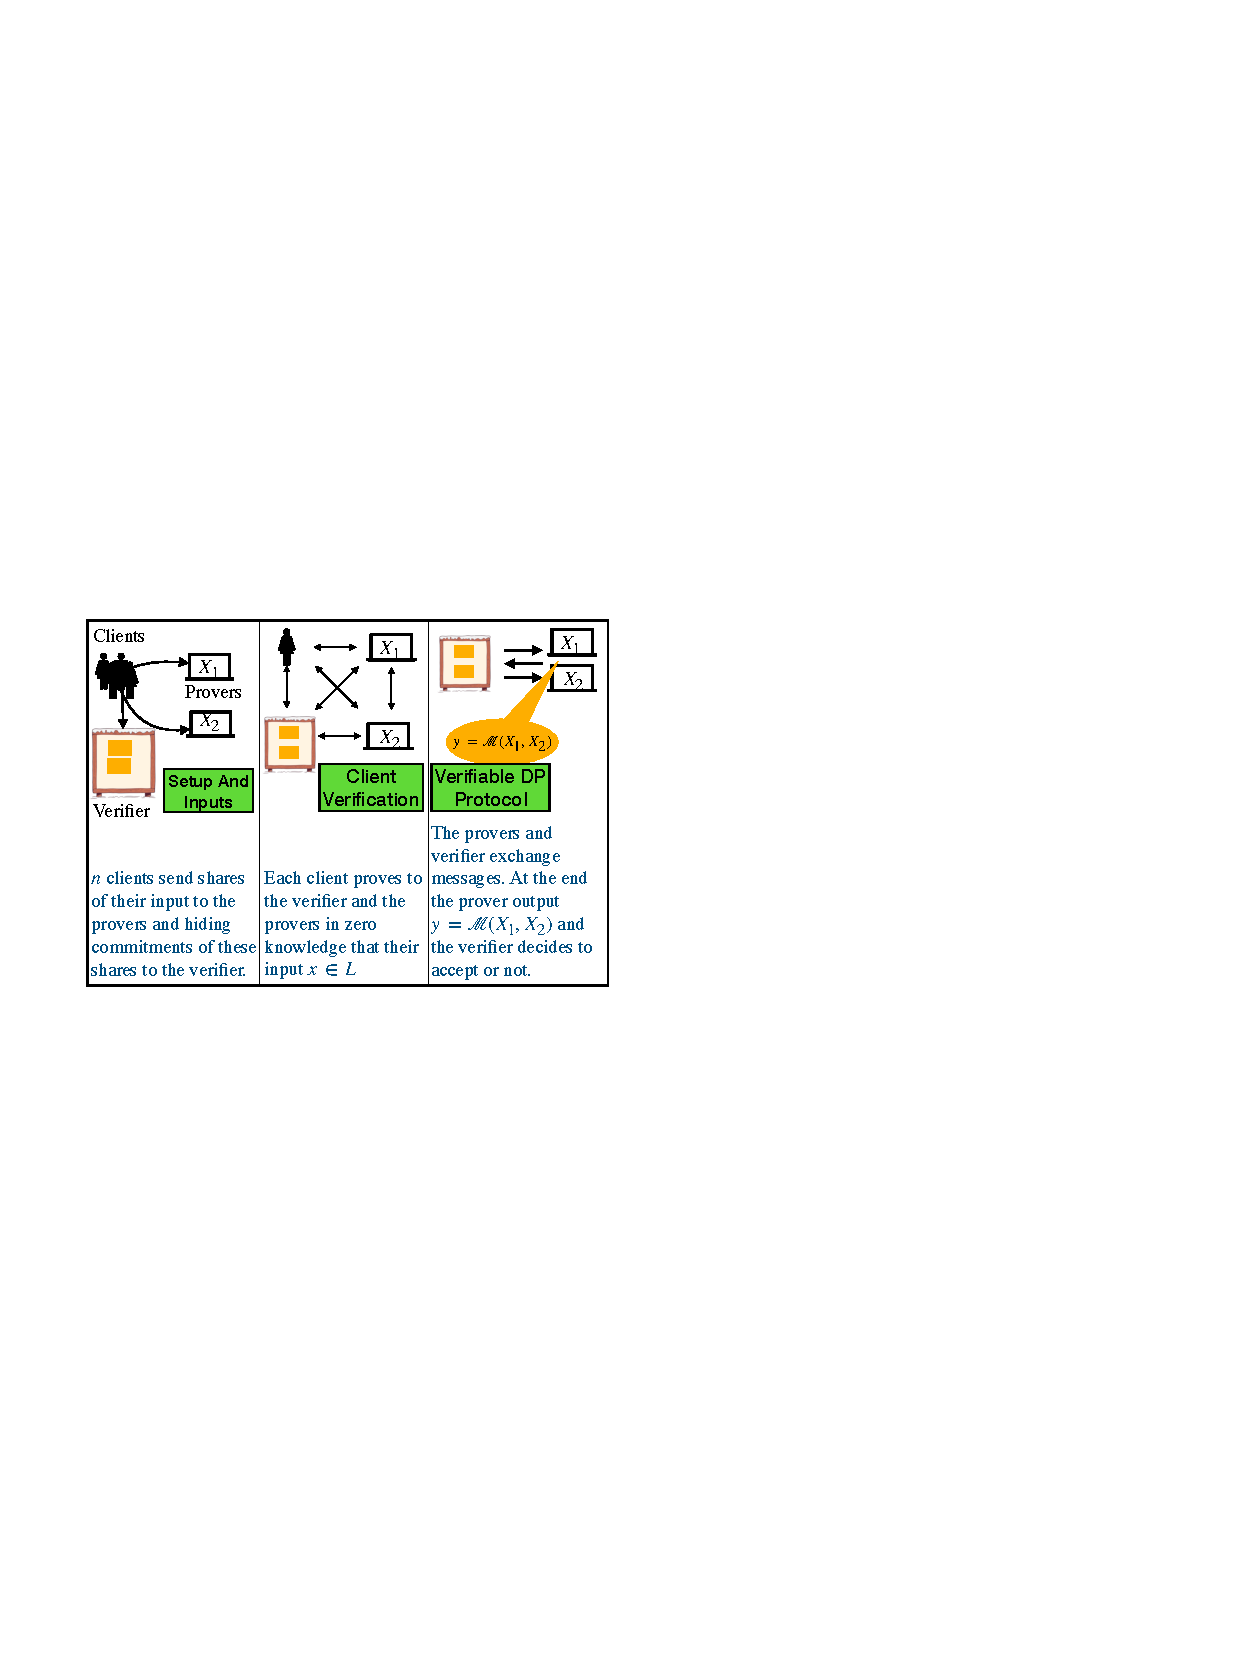
\includegraphics[scale=0.9]{pngs/data_flow.pdf}
%	\caption{The figure above describes the three stages of the protocol.  Any message sent and received by the verifier is accessible to all clients and provers. In the setup stage, public parameters are generated, and each client $i \in [n]$ sends inputs to the prover and the verifier.  In the verification stage, each client interactively exchanges messages with the verifier and the provers to establish their private input $x \in L$ in zero knowledge. If a client fails to do so, they are tagged as dishonest and excluded from the protocol. In the last stage, each prover samples private randomness and then interactively exchanges messages with other provers and the verifier to jointly compute $y = \mathcal{M}_Q(X_1, \dots, X_K)$ for some common knowledge query $Q$.
%	The verifier validates that the provers' output $y$ was computed as prescribed over the inputs of honest clients only. }
%	\label{fig:flow}
%\end{figure}


This section introduces definitions for interactive proofs for differential privacy. The definitions apply to both the single curator and MPC setting.
In both settings, we will assume that the inputs comes from $n$ distinct clients.
Informally, the main difference between the two
models is that the single curator has plaintext access to the client data $X = (x_1, \dots, x_n)$. 
In contrast, in MPC-DP, the client's secret share (or partition) their inputs and each server receives information theoretically hiding shares (or a partial view) of client inputs. 
Additionally, for a given query $f \in \FuncFamily$, instead of having a single entity responsible for outputting samples from $\Mechanism(X, f)$, the servers participate in an MPC protocol denoted by $\Pi$ to securely sample from $\Mechanism(X, f)$.
For some queries $f \in \FuncFamily$, the specifications may require that the client inputs come from a restricted subset $L \subseteq \FuncDomain$.
For such cases, the clients must prove in zero-knowledge to an independent verifier that their inputs come from the specified language without revealing any other information about their inputs. Going back to our pizza topping example in Section \ref{sec:introduction}, the client must prove that they voted for at most one option at most one time.  
Examples of such proofs can be found in the prior literature~\cite{boneh_lightweight_2022,
  boyle2019secure, corrigan-gibbs_prio_2017, bunz2018bulletproofs}.
In the definitions below and in what follows, we use the terms $\Prover$
(prover), server and curator interchangeably, and the terms analyst and
$\Verifier$ (verifier) to refer to the same entity. Unless otherwise specified, for $K \geq 1$, it is safe to assume that the provers $\vec{\Prover} = (\Prover_1, \dots, \Prover_K)$ and verifier $\Verifier$ are PPT Turing Machines.

%\input{tex_files/single_curator_dp_defs.tex}
\subsection{Verifiable DP}

\paragraph{MPC Model}
Next, we describe the MPC model and later discuss how the single curator model is a special case of the general model.
Let $\Mechanism$ be a DP (or IND-CDP) mechanism as described in Definition~\ref{def:dp_approx_definition} (or Definition~\ref{def:comp_dp_definitions} respectively) for a query $f$.  
Let $\SecurityParam \in \Naturals$ denote the security parameter and $n=\lceil\poly(\SecurityParam)\rceil$ denote the number of inputs to the DP mechanism. Let $K \geq 1$ denote the number of provers. A verifiable DP mechanism for $\Mechanism$  consists of a PPT algorithm $\Setup$  and an interactive proof system $\Pi$, between $K+1$ ``next-message-computing-turing machines'' $\Verifier$ and $(\Prover_1, \dots, \Prover_K)$. 
In next-message computing-turing machines, any party, for example, $\Verifier$'s message $m_i$ at round $i$ is determined by its input, messages it has received so far from other parties and internal randomness $\vec{r}_\Verifier$.  
Let $\vec{\Prover}$ denote a succinct representation for $(\Prover_1, \dots, \Prover_K)$. 
$\pp \samples \Setup(1^\SecurityParam)$ describes the PPT algorithm that receives a unary representation of the security parameter $\SecurityParam$ as input and generates public parameters $\pp$ that are broadcasted to all parties.

$\Pi$ describes a multi-prover interactive proof system for differential privacy between $K$ provers and a single verifier. In a multi-prover interactive proof system, the provers and verifier exchange messages for $\poly(\SecurityParam)$ rounds. Let $z \in \bit^{\poly(\SecurityParam)}$ denote auxiliary input available to the verifier $\Verifier$. In a specific rounds\footnote{These rounds need not be the last round of the proof. A proof system may prescribe that the prover send a message tagged as the output and continue to exchange messages in future rounds.} of message exchanging, each prover $\Prover_j$ sends to the verifier $\Verifier$ special messages $y_j$ tagged as the output. Once the verifier has received output messages from every prover, it uses a pre-specified deterministic polynomial time algorithm $A$ to compute $y = A(y_1, \dots, y_k)$. As for all $j \in [K]$, $y_j$ is computed as a function of $\Prover_j$'s internal randomness, $y$ can be viewed as a random sample from the distribution $\Pi(\Verifier, \vec{\Prover}) \in \Delta(\FuncRange)$. Once all messages have been exchanged, the verifier $\Verifier$,  outputs either 0 or 1, with 1 indicating that the verifier accepts the provers' claim that $\Mechanism(X, f)=\Pi(\Verifier, \vec{\Prover})$ and $y$ is a sample from $\Mechanism(X, f)$, and 0 indicating otherwise.

Let $\Output\Big[\Verifier(\pp, \vec{r}_\Verifier, z), \vec{y}, \vec{\Prover}(X, \pp, \vec{r}_{\vec{\Prover}})\Big] \in \bit$ denote the verifying algorithm's decision.
In the definition below, we write $\Output(\Verifier, \Prover)$ as shorthand for the verifier output.
%In $\texttt{Setup}$, all parties jointly generate public parameters and the provers and verifier receives inputs from $n$ clients. 
%Let $ \texttt{Setup}(1^\SecurityParam)$ denote public parameters. 
%Each prover $\Prover_k$ receives on its input tape $n$ secret shares of client inputs $\Big(\share{x_1}_k, \dots, \share{x_n}_k\Big)$, succinctly denoted by $\vec{X_k}$.
%The verifier receives hiding commitments of the above shares. All messages sent and received by the verifier are accessible to all other parties. \par
If the query $f$ restricts client inputs to a subset $L \subseteq \mathcal{X}$ then in $\texttt{Verify}$ phase, the clients interactively exchange messages with the provers and the verifier to prove in zero knowledge that their private input $x \in L$. If clients fail to do so, they are excluded from the protocol. 
Once dishonest clients with illegal inputs have been excluded and honest client inputs have been recorded, the clients play no further role in the protocol. \par



\paragraph{Single Curator}
The single curator can be understood as
essentially the above model with a single prover, i.e., we set $K=1$.  Thus
the only functional difference between MPC-DP and trusted curator DP
is that in the latter case, the curator sees all client inputs in plaintext. 
In MPC, the data may be secret, shared or partitioned
across the provers. 
In both cases, the prover(s) must prove they did not tamper with the protocol to sample an output from a distribution that is different from that specified by $\Mechanism$ \footnote{When there is a single server only, and the client inputs come from a restricted set $L$, although the server can see inputs in plaintext, the verifier cannot. Thus, to prevent malicious clients from colluding with the server, the clients still need to prove to the verifier with zero-knowledge that the inputs are legal.}. Figure \ref{fig:flow} summarises the information flow between the parties.

\statetheoremsolid{0.95\textwidth}{
\begin{definition}[Interactive Proofs For DP]\label{defn:vdp_MPC}
 Fix $\SecurityParam \in \Naturals$ as the security parameter. Let $\Mechanism$ be a DP (or CDP) mechanism for computing $f$ using inputs $X=(x_1, \dots, x_n)$ received from $n$ distinct clients (input sources). Let $K \geq 1$ and $(X_1, \dots, X_K)$ denote a partitioning/secret sharing of $X$ such that there exists a public deterministic PPT reconstruction algorithm $A$, such that $X = A(X_1, \dots, X_K)$.  An interactive proof for verifying $\Mechanism$ consists of a PPT algorithm $\Setup$ and a multi-prover (single if $K=1$) interactive proof system $\Pi$. $\pp \samples \Setup(1^\SecurityParam)$ describes the PPT algorithm that receives a unary representation of the security parameter as input and generates public parameters $\pp$. $\Pi$ denotes a multi prover interactive proof system between, $K \geq 1$ provers $\vec{\Prover}=(\Prover_1, \dots, \Prover_K)$ and a single verifier $\Verifier$ where for each $j \in [K]$, $(X_j, \vec{r_{\Prover_j}}, \pp)$ denotes the inputs for $\Prover_j$ and $(\vec{z}, \vec{r}_\Verifier, \pp)$ denote the verifiers input. Here where $\vec{r_{\Prover_j}}$ and $\vec{r_{\Verifier}}$ denotes $\Prover_j$'s and the verifiers internal randomness respectively and $\vec{z}$ denotes the verifiers auxiliary input. The proof system $\Pi$ is an interactive proof system for mechanism $\Mechanism$ if there exists negligible functions $\delta_c$ and $\delta_s$ in $\SecurityParam$ such that the following hold:

\begin{enumerate}
\item{\textbf{Completeness:} Let $\Pi(\vec{\Prover}, \Verifier)$ denotes the induced output distribution from which the verifier samples the final output $y \samples \Pi(\vec{\Prover}, \Verifier)$ if the verifier and all provers are honest. If $\TV{(\Pi(\vec{\Prover}, \Verifier) , \Mechanism(X, Q))} =0$

    
     \[ \Pr\left[ \texttt{out}(\Verifier, \vec{\Prover}) = 0 : \begin{array}{c} \pp \samples \texttt{Setup}(1^\kappa) \\
      \Prover_j \gets (X_k, \vec{r}_{\Prover_j}, \pp)\\
     \Verifier \gets (\vec{z}, \vec{r}_\Verifier, \pp) \\
y \samples \Pi(\vec{\Prover}, \Verifier) 
    \end{array} \right]
  \leq \delta_c . \] 
  }

\item{\textbf{Soundness:} For any
    subset, $I \subseteq [K]$, let $\vec{\ChProver}$ denote the collection
    of corrupted provers, indexed by $I$,  that deviate from $\Pi$, and $\vec{\Prover}$  denote the set of honest provers not indexed by $I$. Let $\Pi(\vec{\Prover}, \vec{\ChProver}, \Verifier)$ denote the induced output distribution from which the verifier samples the final output $y \samples \Pi(\vec{\Prover}, \vec{\ChProver}, \Verifier)$. Then, if $\TV{(\Pi(\vec{\Prover}, \vec{\ChProver}, \Verifier), \Mechanism(X, Q))} >0$

     \[ \Pr\left[ \texttt{out}(\Verifier,\vec{\Prover}, \vec{\ChProver}) = 1 : \begin{array}{c} \pp \samples \texttt{Setup}(1^\kappa) \\
      \Prover_j \gets (X_k, \vec{r}_{\Prover_j}, \pp)\\
     \Verifier \gets (\vec{z}, \vec{r}_\Verifier, \pp) \\
y \samples \Pi(\vec{\Prover}, \vec{\ChProver}, \Verifier)
    \end{array} \right]
  \leq \delta_s . \] 
  
\ariInline{There is room for interactive proofs for proximity here. Talk to Graham or Vadhan.}  

}
     
\item{\textbf{Zero Knowledge}:  Let $\ChVerifier$ denote an arbitrary verifier strategy that corrupts any proper subset $I \subset [K]$ of provers. 
Let $\vec{\ChProver}$ denote the collection of corrupted provers, indexed by $I$, and $\vec{\Prover}$  denote the set of honest provers.  Let
    $\View\Big[\Pi\Big((\vec{\Prover}, \vec{\ChProver})
    ,\ChVerifier\Big)\Big]$ be the joint distribution\footnote{As
      $\Mechanism$ is a random function, the \highlight{joint
        distribution} of the view of the adversary and \highlight{their output}
      must be indistinguishable from the simulated transcript (and not
      just the view of the adversary). See \cite{lindell2017simulate}
      for more details.} of exchanged messages and induced output distribution $\Dist$ during the
    execution of $\Pi$ in the presence of corrupted parties. There
    exists a PPT algorithm called $\Simulator^{(\ChVerifier, \vec{\ChProver}, \Dist)}$ with black box access to $\ChVerifier$ and $\vec{\ChProver}$ and sample access to $\Dist$, such that if $\TV{(\Dist, \Mechanism(X, Q))}=0$
    
    
    \begin{align*}
\View\Big[\Pi\Big((\vec{\Prover}, \vec{\ChProver})
    ,\ChVerifier\Big)\Big] &\stackrel{}{\equiv} \Simulator^{(\ChVerifier, \vec{\ChProver}, \Dist)}(\vec{r}_\Verifier, \vec{z})        
    \end{align*}
 }

\end{enumerate}
 \end{definition}
}

 Verifiable DP, just like interactive zero knowledge proofs \cite{goldreich_foundations_2007} comes in 24 different flavours based on the capabilities of the corrupted parties:
 
 \begin{enumerate}
 	\item{\textbf{Distinguishability:} Based on the distinguishability properties of the simulator algorithm, the protocol may be perfect, statistical or computationally zero knowledge. The protocol described in Section \ref{sec:single_curator_hist} is computationally zero knowledge. } 
 	\item{\textbf{Verifier specifications:} Based on whether the verifier is expected to follow the rules of the protocol (semi-honest) or may deviate arbitrarily (active), we get honest-verifier zero knowledge or malicious verifier zero knowledge. All our results are malicious verifier zero knowledge.}  	
 	\item{\textbf{Soundness:} Based on the power of the corrupted provers, the proof may be computationally sound (also known as arguments) or statistically sound (secure against unbounded provers). The verifiable DP protocol in Section \ref{sec:single_curator_hist} is computationally sound.}  	
 	\item{\textbf{Inputs:} Based on whether the verifier has access to the auxiliary input, the protocol could be plaintext zero knowledge or auxiliary input zero knowledge. Our protocols allow for the verifier to have auxiliary input.}  	 	
 \end{enumerate}

 
\begin{remark}
 Contrary to soundness, for zero knowledge to hold, the simulated transcript should be indistinguishable from the actual protocol transcript, based on the inputs adversaries used and not the ones the clients sent to a set of corrupted provers.	
\end{remark} 
 
 \begin{remark}
 An interesting point to note is that here verifier plays a dual role. An honest verifier ensures
 that the output is faithfully generated and thus plays an active role in noise generation without ever knowing the value of the random variable.	 On the other hand, a dishonest verifier tries to tamper with the protocol to breach privacy. 
  In non-verifiable DP, the analysts
 (verifier) only has sample access to the induced distribution. They have no agency over how this distribution is constructed. Thus the verifier
 participating in verifiable DP has a greater attack surface than a classical adversary in traditional non-verifiable DP. 
 We elaborate on this in Section \ref{sec:separation}, when trying to establish separations between statistical DP and computational DP.
 \end{remark}
 
 \begin{remark}
Just like in standard MPC, in the presence of a dishonest majority of corrupted participants, we do not treat early exiting by corrupted parties as a breach of security. This is easily detected by the honest parties, and the output is ignored. 	
 \end{remark}
 

\section{Verifiable Binomial Mechanism}
\label{sec:single_curator_hist}

This section describes how to compute counting queries verifiably with differential privacy in both the single curator and client-server MPC models. 
We consider the trusted curator model to be a special instantiation of the general MPC model where the number of provers $K=1$.
In Section \ref{sec:intuition} we describe intuitions for our protocol, and in Section \ref{sec:client-server-mpc-dp} we explain what is needed for verifiability in the MPC setting and tackle the additional challenges of verifying client inputs.
We describe how prior efforts at verifying clients fall short of the security expectations of Definition~\ref{defn:vdp_MPC}. 
Finally, in Section \ref{sec:main_protocol}, we describe a protocol that verifiably computes counting queries with DP.

Set $\mathcal{X} = \Z_q = \mathcal{Y}$, where $\Z_q$ is a prime order finite field of size $q$ over the integers. Let $X=(x_1, \dots, x_n)$ denote the client inputs and  $Q$ be the counting query $Q(X) = \sum_{i=1}^n x_i$.  Let $\share{x_i}_k$ denote the $k$'th additive secret\footnote{Although we describe our protocols with additive secret sharing, any linear secret sharing such as Shamir's secret sharing also applies to all our results.} share of a client input $x_i$. Each client splits their input into $K$ secret shares and distributes them across the provers. We will assume that $n\ll q$ and $\kappa= \lfloor \log_2 q\rfloor$ can be viewed as the security parameter. For $K \geq 1$ provers and 1 verifier, define the oracle functionality $\Mechanism_\bin$ in the ideal world as follows:
%
\begin{enumerate}
	\item{$\mathcal{M}_{\bin}$ receives public privacy parameters $\epsilon$ and $\delta$. It then computes $\noisen$ (number of coins for binomial noise) based on Lemma \ref{theorem:dp_guarantee}.}

	\item{Let $\Big(\share{x_1}_k, \dots,\share{x_n}_k\Big)$ denote the inputs on the $k$'th prover's input tape. Each prover $\Prover_k$  is expected to compute $X_k = \sum_{i=1}^n \llbracket x_i \rrbracket_k$ and sends to $\Mechanism_{\bin}$ as its input $X_k$. A corrupted prover might send an arbitrary input.} 
	
\item{$\Mechanism_{\bin}$ samples $\Delta_k \sim \texttt{Binomial}(\noisen, 1/2)$ independently for each input $X_k$ it receives. It then computes 
%
\begin{equation}
\label{eq:M_bin}
\textstyle
y =  \sum_{k=1}^K (X_k + \Delta_k)
\end{equation}
%
}
\item{$\mathcal{M}_{\bin}$ sends the tuple $(y, \Delta_k)$ as output to each prover $\Prover_k$. On receiving its output, the $\Prover_k$ sends $\texttt{CONTINUE}$ to $\Mechanism_{\bin}$. Once $\Mechanism_{\bin}$ receives the continue signal from prover $\Prover_k$ it moves on to deliver output to $\Prover_{k+1}$.}

\item{After all $K$ provers have sent $\texttt{CONTINUE}$, $\Mechanism_{\bin}$ sends $y$ as output to the verifier $\Verifier$. If a single prover fails to send the continue message and thereby exits the protocol early, the verifier and the remaining provers do not receive any output.}

\end{enumerate}

When $K=1$, i.e., the trusted curator setting, the single prover receives $n$ client inputs in plaintext, so $\share{x_i}_k = x_i$ for all $i \in [n]$. 
This is equivalent to an adversary corrupting all $K$ provers. Thus in the MPC setting with $K \geq 2$ servers, it is safe to assume at least one of them will follow the protocol.
Our goal is to be able to come up with an interactive protocol $\Pi_\bin$, 
that allows us to compute $\mathcal{M}_{\texttt{Bin}}$ verifiably as per Definition~\ref{defn:vdp_MPC}. 
Notice that in the ideal model definition above, the oracle adds $K$ independent copies of DP noise to the output, whereas 
 Lemma \ref{theorem:dp_guarantee} only calls for a single copy. 
 This is because, as we allow up to $K-1$ provers to collude with a corrupted verifier, the corrupted provers could simply not add any noise to the output. 
Ben Or \etal's completeness results  \cite{ben2019completeness} imply that $K$ independent copies of noise are \textit{necessary} to guarantee differential privacy unless the number of corruptions can be restricted to being strictly less than $\frac{K}{3}$, so each prover must independently generate enough noise to guarantee DP.
Our protocols defined below are secure against computationally bounded provers and verifiers that may deviate arbitrarily from protocol specifications and have access to auxiliary inputs.

\subsection{An Intuitive But Incomplete Protocol}
\label{sec:intuition}

Before describing the entire protocol in Section \ref{sec:main_protocol} and Figure \ref{fig:dp_interactive_proof}, we provide the reader with some intuition as to why the protocol works for a single curator and verifier. \textit{In this section, we make the unrealistic assumption that prover and verifier behave faithfully}. 
Assume all parties have joint oracle access to $\oracle_{\Morra}$ (as described in Section \ref{sec: morra}) to jointly sample unbiased bits $(b_1, \dots, b_{\noisen})$. It is easy to see that using $(\sum_{i=1}^{\noisen} b_i)$ as DP randomness results in the desired Binomial distribution defined in $\mathcal{M}_{\texttt{Bin}}$. However, the oracle output is known to both the verifier and prover; therefore, it cannot be directly used to guarantee differential privacy. 
As discussed earlier, this problem of proving that a prover faithfully sampled random bits without disclosing them lies at the heart of any verifiable DP protocol. 
Thus the protocol must combine public coins that satisfy verifiability requirements and private coins that ensure secrecy.

The protocol for verifiable DP counting proceeds in $\noisen$ identical and independent invocations (run in parallel). 
In copy $i$, the prover samples $v_i \in \bit$, which it keeps private. 
Note that a prover could sample this bit using any arbitrary bias. 
As this is the provers' private coin, the verifier has no control over how the prover generates this information. 
After the prover has sampled their private bit, the prover and verifier make one call to $\oracle_{\Morra}$ to get an unbiased coin denoted by $b_i$. 
Next, the prover locally computes  $\hat{v}_i = b_i \oplus v_i$. Here $\oplus$ refers to the boolean XOR operation. It is easy to see that $\hat{v}_i$ has the same distribution as $b_i$, but its value is known only to the parties with access to $v_i$, i.e., the prover. 
After $\noisen$ rounds, the prover computes $Q(X)$ and $Z = \sum_{i=1}^{\noisen} \hat{v}_i$ and outputs $Q(X) + Z$ where $Z$ is used as DP randomness.  By the assumption that the prover and verifier are faithful, $Z$ is distributed according to the desired distribution stated in Theorem \ref{theorem:dp_guarantee}, and its value is only known to the prover. 
To make this protocol practical, we need to resolve a few issues.

\begin{enumerate}
    \item{Although the above description requires a bitwise XOR operation to ensure the right distribution is used, we operate with arithmetic circuits in the actual protocol. 
    Thus, the provers could sample arbitrary values $v^* \in \Z_q$ such that $v^* \notin \bit$, and we need to fix how to express the XOR operation via arithmetic circuits. 
   %Secondly, it is not immediately clear what it means to do an XOR operation in arithmetic circuits with non-boolean values.
    }

    \item{Even if we could verify that the prover sampled a private bit correctly, we still need to verify that they faithfully performed the local operations discussed above.}
\end{enumerate}

Thus, if we could guarantee that each server performed its computations correctly and sampled a private value from the correct set, we would get the desired outcome of verifiable and DP counting queries.

\begin{figure}[t]
    \centering    
	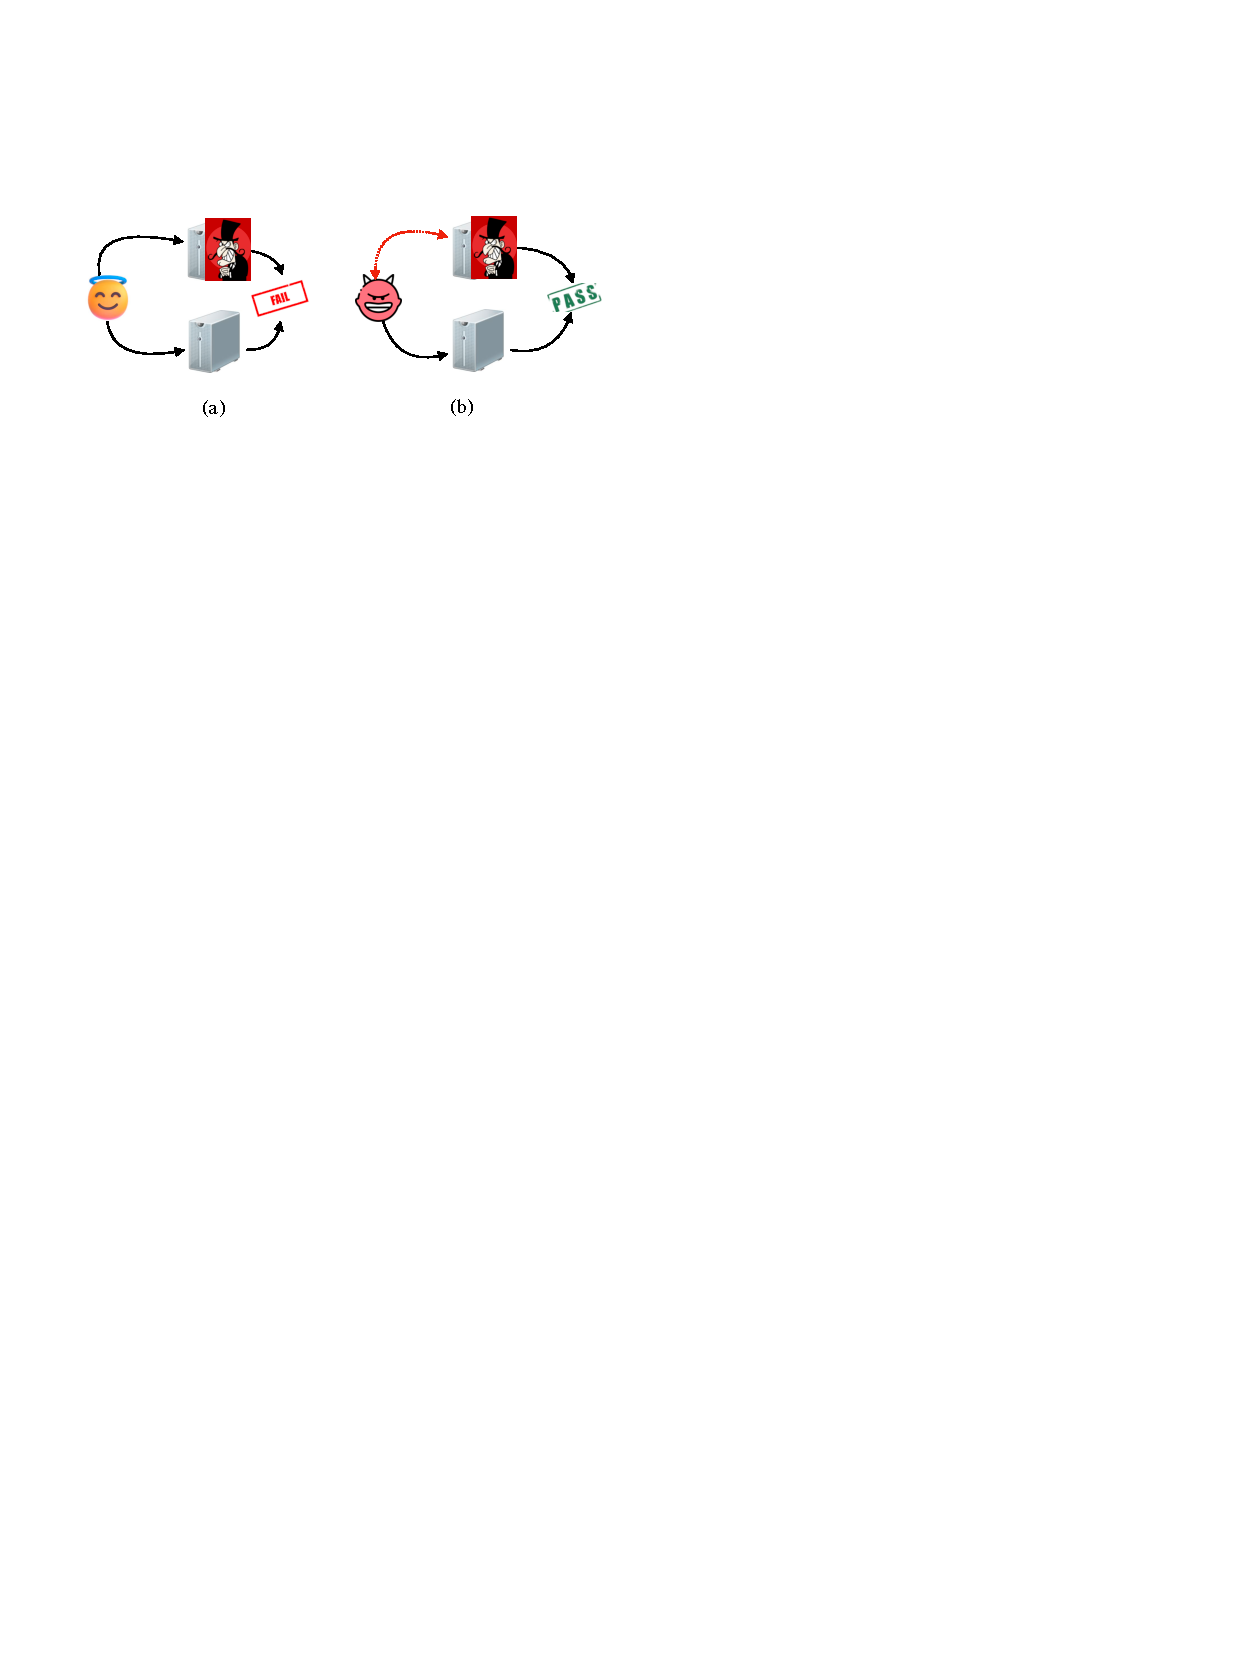
\includegraphics[scale=0.9]{pngs/attack.pdf}
	\caption{Two types of attacks that go undetected in Poplar. In (a) regardless of what the honest client sends, a corrupted server simply ignores the input and excludes the client from the protocol based on auxiliary information. In (b) a dishonest client colludes with the corrupted server by revealing secret values, so that an illegal input is included. In both cases, the honest server cannot distinguish between an honest run and a corrupted run of the protocol.}
	\label{fig:attacks}
\end{figure}

\subsection{Extending To Client-Server MPC-DP}
\label{sec:client-server-mpc-dp}

To compute DP histograms verifiably in the client-server MPC-DP setting, we use the same computational model used for PRIO \cite{corrigan-gibbs_prio_2017} and Poplar \cite{boneh_lightweight_2022}. Prio is deployed at scale by Mozilla \footnote{\url{https://blog.mozilla.org/security/2019/06/06/next-steps-in-privacy-preserving-telemetry-with-prio/}}.
As discussed earlier, in this setting $n$ clients secret share their inputs $x_i \in L$ amongst $K \geq 2$ provers, where $L \subseteq \mathcal{X}$ defines the language of legal inputs to the protocol. 
For computing $M$-bin histograms over $n$ inputs, $L$ is the set of all one-hot encoded vectors of size $M$. 
For the core problem of a single-dimensional counting query, we have $M=1$ and $L=\bit$.  
Since the inputs on the prover's tapes reveal no information about a client's input, for the protocol to be useful the provers must first verify in zero knowledge that $x_i \in L$ before using such inputs to compute aggregate statistics. 
This additional step of verifying a client is not required in the trusted curator model, as the prover decides what inputs should be included in the computation and can see them in plaintext.

\paragraph{Verifying Clients in MPC-DP}
\label{sec:client_verification}

Poplar and PRIO use efficient sketching techniques from \cite{boyle_function_2016} to validate a client's input in zero knowledge \textit{without} relying on any public key cryptography. Thus, as long as at least one out of $K$ provers does not reveal the inputs it received, even an unbounded adversary corrupting the remaining provers cannot ascertain any information about an honest client's input. While such a system protects an honest client's privacy from an unbounded adversary, it is not verifiable as per Definition \ref{defn:vdp_MPC}. 
Specifically, for the techniques used in PRIO and Poplar, a single corrupted prover could tamper with its inputs and exclude an honest client from the protocol by forcing them to fail the verification test. 
Alternatively, a corrupt client could collude with a prover to include arbitrary inputs, jeopardising the correctness of the output. 
Figure\footnote{Content from J.J. at the English-language Wikipedia, licensed under \href{https://creativecommons.org/licenses/by-sa/3.0/deed.en}{CC BY-SA 3.0}.}~\ref{fig:attacks} summarises these attacks on Poplar and PRIO\footnote{Concretely, referring to  notation from \cite[Appendix C]{boneh_lightweight_2022}, in scenario (b), the dishonest client reveals the values $\kappa$ and $[v]_0$ to the server. This allows the server to set $z_1 = -z_0, z_1^* = -z_0^*$ and $z_1^{**} = -z_0^{**}$, thereby 
 admitting an illegal input into the protocol.}. By our definitions of verifiability, the protocol's output \textit{must} be a function of the inputs provided by honest clients only. 
 Thus the protocol described in Section \ref{sec:main_protocol} provides the following additional guarantees:

\begin{enumerate}
	\item{\textbf{Guaranteed Inclusion Of Honest Clients}: If a client submits shares of an input $x \in L$, then the final output of the protocol is guaranteed to use this input untampered. Thus an honest client is assured that, as long as a single prover follows the protocol specifications, no one learns any information about their private input and their input is correctly used to compute the final output. }
	\item{\textbf{Guaranteed Exclusion Of Corrupt Clients}: A corrupted client, even one that has control over any proper subset of the $K$ provers, cannot include an invalid input to the protocol. Thus if $x \notin L$, $x$ is discarded by our protocol with overwhelming probability.}
\end{enumerate}

It is important to note that as we operate under stricter notions of privacy and correctness, our results require the use of public-key cryptography and security holds only against computationally bounded adversaries.  Furthermore, we show in Section \ref{sec:separation} that it is impossible to satisfy verifiable DP and provide information theoretic guarantees.

\begin{figure*}[h]
    \centering
\begin{pchstack}[boxed]  % default  
    \pseudocode[linenumbering , skipfirstln]{%
    \textbf{ Verifier}(\Verifier) \< \< \textbf{Prover}(\Prover_k) \\[][\hline]
    \pp \samples \texttt{Setup}(1^\SecurityParam) \< \text{Generate public parameters} \<   \pp \samples \texttt{Setup}(1^\SecurityParam) \\
	\Bigg\{  \Big\{ c_{i,k}  \Big\}_{k \in [K]} \Bigg\}_{i \in [n]} \< 
 \text{Client inputs }  \<  \Big\{ \share{x_i}_k, r_{i,k} \Big\}_{i \in [n]}, 	\Bigg\{  \Big\{ c_{i,k}  \Big\}_{k \in [K]} \Bigg\}_{i \in [n]}\\
     \forall i \in [n] \text{ Send } c_{i} = \prod_{k=1}^K c_{i,k}  \<  \oracle_{\OR} \<   \forall i \in [n] \text{ Send } c_{i} = \prod_{k=1}^K c_{i,k}\\
\text{For any } i \in [n] \text{ if }\oracle_{\OR}(c_{i}) \neq 1\<\text{Exclude } (\share{x_i}_k, r_{i,k}) \text{ from the protocol} \<  \\
    (c'_{1,k}, \dots, c'_{{\noisen},k})\< \sendmessageleft*{c'_{j,k} = \Com\Big( v_{j,k}, s_{v_{j,k}}\Big)} \< \forall j \in [\noisen] \text{ Samples and commits } v_{j,k} \in \bit \text{}\\    
    \forall j \in [\noisen]\text{ Send } c'_{j,k} \< 
\oracle_{\OR}  \<  \forall j \in [\noisen] \text{ Send openings} (v_{j,k}, s_{j,k})\\    
    \forall j \in [\noisen]\text{ Check } \oracle_{\OR}(c'_{j,k}) = 1\<\<  \\
    \forall j \in [\noisen]\text{ Send empty string } \lambda_j \< 
\oracle_{\Morra} \< \forall j \in [\noisen]\text{ Send empty string } \lambda_j\\
    \text{ Receive } (b_{1,k}, \dots, b_{\noisen,k}) \< 
 \forall j \in [\noisen] \text{ }b_{j,k} = \oracle_{\Morra}(\lambda_j) \text{ } \< \text{ Receive } (b_{1,k}, \dots, b_{\noisen,k})\\  \< \< \forall j \in [\noisen] \text{ Update }v_{j,k} , s_{j,k}  \text{ to get }  \hat{v}_{j, k}, \hat{s}_{j, k} \\
 \<\<\text{ based on }  b_{j,k}\\ 
  \<  \< y_k = \sum_{i=1}^n \share{x_i}_k + \sum_{j=1}^{\noisen} \hat{v}_{j,k} \text{ and } \\
  \< \sendmessageleft*{(y_k, z_{k})} \< z_{k} = \Big(\sum_{i=1}^{n}r_{i,k}+ \sum_{j=1}^{\noisen} \hat{s}_{j,k}\Big) \\  
    \text{Compute } \hat{c}'_{j,k} \text{ using } b_{j,k}  \text{ for all } j \in [b_{\noisen}]\< \<  \\    
  \text{Check } \Big( \prod_{i=1}^{n} c_{i,k} \times \prod_{j=1}^{\noisen} \hat{c}'_{j,k}\Big) \< \< \\
  \qquad = \Com(y_k, z_{k})\< \<
}
\end{pchstack}    
\caption{The figure above describes the interaction between a single prover and verifier in $\Pi_{\bin}$. In the single trusted curator model $K=1$ we have $x_i = \share{x_i}_k$ where the prover can see client inputs in plaintext. In the MPC setting, each prover $\Prover_k$ follows the exact same protocol on their respective inputs specified in Line 2. Thus at the end of the protocol, each prover $\Prover_k$ outputs the tuple $y_k, z_{k}$. A verifier aggregates the output from each prover to publish verifiable DP statistics. }
    \label{fig:dp_interactive_proof}
\end{figure*}


\subsection{Main Protocol Description}
\label{sec:main_protocol}

The protocol $\Pi_{\bin}$ described in Figure \ref{fig:dp_interactive_proof} provides a compact standalone description of the interaction between $K$ provers and the verifier for computing $\Mechanism_\bin$. 
We assume that both the provers and the verifier have access to oracles $\oracle_{\Morra}$ and  $\oracle_{\OR}$ as defined in Section \ref{sec: commitments}. 
In the real world, $\oracle_{\Morra}$ is replaced with $\Pi_{\Morra}$ (see Algorithm \ref{alg: morra}) and $\oracle_{\OR}$ is replaced by Cramer \etal's $\Sigma$-OR proof \cite{cramer1994proofs} (see Appendix \ref{app:sigma_open} for an example implementation) which securely compute the oracle functionalities in the presence of adversaries that may deviate from protocol specifications. Thus, we define our protocol in the hybrid world, and by the sequential composition theorem\footnote{Though we use sequential composition, both protocols $\Pi_{\Morra}$ and $\Pi_{\OR}$ can be composed in parallel.} \cite{goldreich_foundations_2007}, the security properties of the protocol are preserved. 
Next, we describe the protocol in detail with line references to Figure \ref{fig:dp_interactive_proof}:

\begin{enumerate}
    \item[Line 1:]{ In the first step, the prover(s) and verifier agree upon the public parameters for the protocol. The public parameters include a description of $\mathcal{C}_\pp = \G_q, \mathcal{M}_\pp = \mathcal{X} = \mathcal{Y} = \Z_q, \RandomnessSpace_\pp= \Z_q$ and a description of $\mathcal{M}_\texttt{bin}$ as defined in equation \eqref{eq:M_bin}. 
    The group $\G_q$ satisfies the requirements of the homomorphic commitment scheme defined in Section \ref{defn:hom_coms} and we assume that the discrete log problem is hard to solve in $\G_q$.}

\item[Line 2:]{ For each client $i \in [n]$, let $\share{x_i}_k$ denote the $k$'th share of their input $x_i \in L$. 
Define $c_{i,k} = \Com\Big(\share{x_i}_k,  r_{i,k}\Big)$ as the commitment to the $k$'th share of $x_i$. 
The client sends to each prover $\Prover_k$ the tuple $(\share{x_i}_k,  r_{i,k})$ and broadcasts 
the commitments to each of the shares $\Big( c_{i,1}, \dots, c_{i,K} \Big)$ to a public bulletin board that is observable to all parties.}

\item[Line 3-4:]{Similar to PRIO and Poplar, we use $L=\bit$, and thus verifier and the client use the oracle $\oracle_{\OR}$ to check if the client's input is indeed a commitment to a bit. 
For input $x_i$, the verifier (and provers) sends to  $\oracle_{\OR}$ the derived commitment $c_{i} = \prod_{k=1}^K c_{i,k}$ and the client sends the openings $\Big(x_i, \sum_{k=1}^K r_{i,k}\Big)$. 
The oracle responds with $\oracle_{\OR}(c_{i}) = 1$ if $x_i \in \bit$ and $c_i$ is a commitment to $x_i$.
In the real world, we replace $\oracle_{\OR}$ with a $\Sigma$-OR protocol \footnote{In the interactive setting, the verifier, the provers, and the client jointly sample a public challenge by playing Morra. As long a single party is honest, the challenge is guaranteed to be selected uniformly at random. Alternatively, in the ROM model, the client sends to a public bulletin board a non-interactive $\Sigma$-proof using the Fiat-Shamir transform.}. This step resolves the issues presented in Figure~\ref{fig:attacks}, as an honest client cannot be excluded nor can a corrupt client input be included. From here on, the protocol only uses inputs from validated clients.}
%
\item[Line 5:]{$\Prover_k$ samples $(v_{1,k}, \dots, v_{\noisen,k})$ where $v_{j,k} \in \bit$ (private random bit) and sends to the verifier commitments to $v_{j,k}$ for $j \in [\noisen]$. 
    Let $c'_{j,k} = \Com(v_{j,k}, s_{j,k})$ denote the commitment to $v_{j,k}$ with randomness $s_{j,k}$. To enforce consistency in notation and improve readability, we always use $c$ to denote commitments to client inputs and $c'$ to denote commitments to the prover's private inputs. Similarly, we will always use $r$ and $s$ to denote the randomness used for client input and prover bit commitments, respectively.}    
%
\item[Line 6-7:] {The verifier uses $\oracle_{\OR}$ to check if the messages sent by the prover were indeed commitments to 0 or 1 (similar to verifying client inputs). 
This step is essential for the Boolean to arithmetic conversion, as the linearisation of the XOR operation is only valid for values $v \in \bit$ (see completeness property of Theorem~\ref{theorem:verifiable_dp_feasible}).}

\item[Line 8-9:]{If for any $i \in \noisen$, $\oracle_{\OR} = 0$, the verifier aborts the protocol and broadcasts that $\Prover_k$ cheated. Otherwise, once all commitments are verified, the prover and verifier jointly invoke $\oracle_{\Morra}$ to get $\noisen$ \textit{public} unbiased bits $(b_{1,k}, \dots, b_{\noisen,k})$.}

\item[Line 10-11:]{For all $i \in [\noisen]$, based on the value of $b_{j,k}$, the prover sets $\hat{v}_{j,k}$ and $\hat{s}_{j,k}$ as follows
    %
    \[   
    \hat{v}_{j,k} = 
         \begin{cases}
        1 - v_{j,k} & \text{if } b_{j,k}=1\\
        v_{j,k}& \text{otherwise.} \\ 
     \end{cases}
\]

    \[   
    \hat{s}_{j,k} = 
         \begin{cases}
        1 - s_{j,k} & \text{if } b_{j,k}=1\\
        s_{j,k}& \text{otherwise.} \\ 
     \end{cases}
\]

As long as $v_{j,k} \in \bit$, the above set of equations is equivalent to setting $\hat{v}_{j,k} = v_{j,k} \oplus b_{j,k}$. An important feature of this step is that, conditioned on $b_{j,k}$, the operations described above are linear. Line 11 describes why this is critical for correctness to hold.
}

    \item[Line 12-13:]{The prover sends $(y_k, z_{k})$ to the verifier:
    \begin{equation}
    y_k = \Big(\sum_{i=1}^n  \share{x_i}_k + \sum_{j=1}^{\noisen} \hat{v}_{j,k} \Big) 
    \end{equation}    
    \begin{equation}
    z_{k} = \Big(\sum_{i=1}^n r_{i,k} + \sum_{j=1}^{\noisen} \hat{s}_{j,k}\Big)     
    \end{equation}
    
    where $(y_k, z_{k})$ is the output for prover $\Prover_k$.
    }

    \item[Line 14:]{Using the common public randomness $\{ b_{j,k} \}_{j \in [\noisen]}$ generated by $\oracle_{\Morra}$, the verifier updates their view of received commitments as follows:

      \[   
\hat{c}'_{j, k} = 
     \begin{cases}
       \Com(1, 1) \times {c'}_{j, k}^{-1} & \text{ if } b_{j, k}=1\\
       c'_{j, k}&\quad\text{otherwise.} \\ 
     \end{cases}
\]
    Note that $\Prover_k$ never opens $\hat{c}^\prime_{j, k}$, and thus $\Verifier$ never sees $\hat{v}_{j, k}$ in plaintext. By the hiding property of commitments, an efficient verifier learns nothing about the prover's private values from these messages. However, as the update conditioned on $b_{j, k}$ is linear and $b_{j, k}$ is public, $\Verifier$ can still compute a commitment to $1 - v_{j, k}$ without ever knowing $v_{j, k}$. As a direct consequence, as discussed in the soundness claim, the prover cannot deviate from its prescribed linear operation, as the verifier can check it.
    As we will show later, this step guarantees correctness, soundness and security. 
    }
    \item[Line 15-16:]{Finally, the  verifier checks 
    \begin{equation}
    \label{eq:vfr_check}
     \prod_{i=1}^{n} c_{i,k} \times \prod_{j=1}^{\noisen} \hat{c}'_{j, k} = \Com(y_k, z_k)   
    \end{equation}        
    }    
\end{enumerate}

From these outputs, we can derive the desired result: we treat the $y_k$'s as shares, and calculate $y = \sum_{k=1}^{K} y_k$ as the noisy sum.  
We next show that this protocol achieves our desired properties. 
\begin{thm}
\label{theorem:verifiable_dp_feasible} 
Let $X=(x_1, \dots, x_n)$ be the client input. Let $\Mechanism_\bin$ and $\oracle = (\oracle_{\Morra}, \oracle_{\OR})$ be as defined above.  $\Pi_{\bin}$ is a verifiably differentially private argument with perfect completeness, negligible soundness and is computational zero knowledge.

%%then the following is true
%%
%%    \item{\textbf{Completeness:} For every $X \in \mathcal{X}^n$ 
%%%    
%%     \[ \Pr\left[ \texttt{out}(\Vfr, \vec{\Pv}) = 0 : \begin{array}{c} \pp \leftarrow \texttt{Setup}^\oracle(1^\kappa) \\
%%     \Pv_k^\oracle \leftarrow \share{X}_k, \bvec{r}_{\Pv_k}, \pp \\
%%     \Vfr^\oracle \leftarrow z, \bvec{r}_v, \pp \\
%%y \leftarrow \Pi_\bin^\oracle(\vec{\Pv}, \Vfr)
%%    \end{array} \right]
%%  = 0  \] 
%%  
%%  where $\share{X}_k = (\share{x_1}_k, \dots, \share{x_n}_k)$ and $\bvec{r}_{\Pv_k}$ denotes $\Pv_k$'s private randomness.
%%  }
%%
%%\item{\textbf{Computational Soundness:} For every $X \in \mathcal{X}^n$ and any subset $I \subseteq [K]$, let $\vec{\Pv^*}$ denote the collection of provers, indexed by $I$, that have been corrupted by an adversary $\AdvA$, such that the final output $y \neq \Mechanism_\bin(X, Q)$. Let $\vec{\Pv}$ denote the collection of honest provers not indexed by $I$. Let $z$ denote the auxiliary input available to $\AdvA$ and $\mu$ be its advantage in the discrete log game (Definition \ref{defn:discrete_log}) 
%%
%%  \[ \Pr\left[ \texttt{out}(\Vfr, \vec{\Pv^*}, \vec{\Pv}) = 1 : \begin{array}{c} \pp \leftarrow \texttt{Setup}^\oracle(1^\kappa) \\
%%     \Pv_k^\oracle \leftarrow \llbracket X \rrbracket_k, \bvec{r}_{\Pv_k}, \pp \\
%%     \Vfr^\oracle \leftarrow z, \bvec{r}_v, \pp \\
%%y \leftarrow \Pi_\bin^\oracle\Big((\vec{\Pv}, \vec{\Pv^*}), \Vfr\Big)
%%    \end{array} \right]
%%  \leq \mu(\kappa)  \] 
%%  
%%Note that as $I \subseteq [K]$, soundness, as defined above, covers both the MPC and the trusted curator setting.
%%}
%%     
%%    \item{\textbf{Computational zero knowledge}: 
%%Let $\vec{\Pv^*}$ denote the collection of provers, indexed by $I \subset [K]$, that have been corrupted by a corrupt verifier $\Vfr^*$. There exists a PPT Simulator $\Sim_{(\Vfr^*, I)}$ such that for all $y = \mathcal{M}(X, Q)$
%%    \begin{align*}
%%    \texttt{View}\Bigg[\Pi\Big((\vec{\Pv}, \vec{\Pv^*}), \Vfr^*, \pp\Big)\Bigg] &\stackrel{c}{\equiv} \Sim_{(\Vfr^*, I)}(y, \bvec{r}_v, z, \pp)        
%%    \end{align*}
%%
%%    Where $z \in \bit^{\texttt{poly}(\kappa)}$ and $\bvec{r}_v \in \bit^{\texttt{poly}(\kappa)}$ represents auxiliary input and randomness available to all the corrupted parties.
%%    }
%
%
\end{thm}

\begin{proof}
\

\paragraph{\textbf{Completeness:}}
By the definition of $\oracle_{\Morra}$, $(b_{1,k}, \dots, b_{\noisen,k})$ are all unbiased bits. 
As per $\Pi_{\bin}$, when $b_{j,k}=1$, $\hat{v}_{j,k}=1-v_{j,k}$ and when $b_{j,k}=0$, $\hat{v}_{j,k} = v_{j,k}$. 
We know that an honest prover is guaranteed to have sampled a private value $v_{j,k} \in \bit$ for all $j \in [\noisen]$. 
Thus the case-wise arithmetic operation described above is equivalent to setting $\hat{v}_{j,k} = v_{j,k} \oplus b_{j,k}$. 
This implies that for each server $\hat{v}_{j,k} \xleftarrow{R} \bit$ and $\sum_{j=1}^{\noisen} \hat{v}_{j,k} \sim \texttt{Binomial}(\noisen, 1/2)$. 
The output of each honest prover is thus $y_k = \texttt{Binomial}(\noisen, 1/2) + \sum_{i=1}^n \share{x_i}_k$. 
By linearity of secret-sharing, $\sum_{k \in [K]} y_k = \mathcal{M}_{\bin}(X, Q)$ where  $\mathcal{M}_{\bin}$ is defined in equation \eqref{eq:M_bin}. 

\paragraph{\textbf{Soundess}}
Beyond exiting the protocol early (which is trivially detected), an adversary $\AdvA$ controlling a collection of dishonest provers could force a prover to cheat by doing at least one of the following:

\begin{enumerate}

    \item{ (Cheat at Line 4): For any $j \in [\noisen]$, $c'_{j,k}$ is not a commitment to a bit. As the verifier has access to oracle $\oracle_{\OR}$, it would detect this immediately. Thus we can be guaranteed that $c'_{j,k}$ are commitments to 1 or 0.}

    \item{(Cheat at Line 7): The prover could sample improper public randomness. 
    However, this is impossible as the verifier and prover jointly use $\oracle_{\Morra}$ to generate randomness.}
    
    \item{(Cheat at Line 13): Output messages $(y_k^\prime \neq y_k$, $z_{k}^\prime \neq z_{k})$. 
    If the verifier check from (Line 15) fails then the verifier knows $\Prover_k^*$ cheated. If 
      $\Com(y_k, z_{k}) = \prod_{i=1}^{n} c_{i, k}\times \prod_{j=1}^{\noisen} \hat{c}'_{j,k} = \Com(y_k^\prime, z_{k}^\prime)$, then $\AdvA$ has broken the binding property of the commitment scheme. As $\AdvA$ has negligible success in winning the discrete log game, it has a negligible chance at breaking the commitment scheme. 
    }
\end{enumerate}

These are the only places where the $\ChProver$ sends a message to the $\Verifier$, and thus we have our result.

\paragraph{\textbf{Zero Knowledge}}

To prove zero knowledge, we need to define the commitment scheme we are using explicitly. We use Pedersen Commitments, which are defined as follows 
\begin{equation}
\label{eq:ped_com}
    \Com(x, r) = g^xh^{r}
\end{equation}
\noindent
where $\RandomnessSpace_\pp = \mathcal{M}_\pp= \Z_q$ and $\mathcal{C}_\pp = \G_q$ is an abelian group where the discrete log problem is hard. To enhance readability, we will prove security for  $K=2$ provers and one verifier, but the result trivially generalises to $K \geq 2$ provers. To avoid confusion between the MPC and single curator setting, we defer the simpler security proof for single curators to Appendix \ref{app:single_curator_sec_proof}. 
Without loss of generality, assume that the verifier $\ChProver$ and $\Prover_1$ have been corrupted by a PPT adversary $\AdvA$ and that $\Prover_2$ is honest. 
$\Simulator$ receives on its input tape the inputs for $\Prover_1$ and $\Verifier^*$. The ideal oracle functionality $\Mechanism_\bin$ is defined as before. Let $\Simulator$ denote shorthand for $\Simulator_{\ChVerifier, \Prover_1}$.  We construct the simulator as follows:

\begin{enumerate}
    
    \item{$\Simulator$ receives the public messages $\Bigg\{  \Big\{ c_{i,k}  \Big\}_{k \in [K]} \Bigg\}_{i \in [n]}$ and sets $c_{i} = \prod_{k=1}^K c_{i,k}$.}

    \item{$\Simulator$ internally invokes $\Prover_1$ to receive inputs $X_1$. If $\Prover_1$ was honest then $X_1 = \sum_{i=1}^n \llbracket x_i \rrbracket_1$. Of course, we have no control over $\AdvA$, and $X_1$ could be any arbitrary value. The definition of security requires that we prove security using the actual inputs used by the real-world adversary $\AdvA$ and not the ones it was handed to at the start of the protocol.}

    \item{$\Simulator$ invokes $\Mechanism_\bin$ with input $X_1$ and receives $(y, \Delta_1)$ as defined in equation \eqref{eq:M_bin}. Note $\Simulator$ never has access to the honest party's input $X_2$ nor the randomness $\Delta_2$ used by $\Prover_2$ in the real protocol. It must simulate the messages and output of the real protocol from just its input and the output it receives from the ideal model.}

    \item{$\Simulator$ sets $y_1= X_1 + \Delta_1$ and computes $y_2 = y - y_1$, which by the definition of $\Mechanism_\bin$, is equal to $(X_2 + \Delta_2)$.}

    \item{$\Simulator$ samples $z_2 \samples \RandomnessSpace_\pp$ and sets $c_{2} = \Com(y_2, z_{2})$.}

    \item{$\Simulator$ samples $c'_{2,2}, \dots, c'_{{\noisen},2}$ such that $c'_{j,2} = \Com(1, s_{j,2})$ where $s_{j,2} \samples \RandomnessSpace_\pp$. 
     It sets $c'_{1,2} = g^1a_2$ where $a_2 = c_{2} \times  \Big( \prod_{j=2}^{\noisen} \hat{c}'_{j,2}\Big)^{-1} \times \Big( \prod_{i=1}^{n} c_{i,2}\Big)^{-1} \times g^{-1}$. 
     Notice that $\Simulator$ is actually unable to open $c'_{1,2}$ but is never required to do so, as opening a commitment to a private value violates DP. The only information $\AdvA$ can check is if $c'_{1,2}$ is a commitment to a bit, which it is. Thus the simulator artificially constructs a set of commitments that align with the real-world protocol, without having the slightest idea what the randomness used by $\Prover_2$ actually was. It is able to do so due to the hiding property of the commitment scheme.}
    
     \item{$\Simulator$ sends over $\{c_{j,2}\}_{j \in [\noisen]}$ to $\AdvA$ pretending to be the honest prover (Line 4 of Figure \ref{fig:dp_interactive_proof}).}
	    
    \item{$\Simulator$ pretends to be the prover and jointly invokes $\oracle_{\Morra}$ with $\AdvA$ to sample $\noisen$ unbiased public bits $(b_{1,2}, \dots, b_{\noisen,2})$.}
    
    \item{$\Simulator$ sends $y_2$ and $z_{2}$ to $\AdvA$ and outputs whatever $\AdvA$ outputs.}
    \end{enumerate}
\end{proof}
%
\subsection{Public Verifiability and Randomness}

Notice that the verifier does not contribute a private input to the protocol, and its messages contain no private information either. 
Furthermore, any party (the clients or the prover) may view the messages sent and received by the verifier.
The verifier's role is primarily to generate unbiased public randomness (independent of the prover's messages), which is used to ensure soundness. 
It samples a challenge for the $\Sigma$-OR proof to verify that the prover's private values are well formed.
Additionally, it participates in Morra, to generate unbiased public coins to enforce the prover's DP noise is sampled from the correct distribution. 
In the computational complexity literature, such a verifier is called a public coin verifier \footnote{\url{https://en.wikipedia.org/wiki/Interactive_proof_system}}. 
If there was another way to sample unbiased and reliable randomness without the verifier, anyone accessing the message transcript could verify if soundness holds.  Consider the Random Oracle Model (ROM), where the verifier's randomness generation (Morra) is replaced by applying a random oracle on the prover and client messages.
Further, consider that all messages from the prover(s) are sent to a public bulletin board along with the client's input commitments and timestamps, with the slight modification that the prover sends commitments and non-interactive proofs of validity \textit{before} the clients send messages to the board. 
The order matters as this prevents the prover from adaptively selecting private values based on the clients' messages, thereby biasing the output of applying a ROM on the board's contents. This way, the prover's messages are guaranteed to be independent of the honest client's messages.
Now, any party (including the clients or even one that did not participate in the protocol) can verify that the randomness is correctly generated (using the oracle on the bulletin board messages) and then perform the checks assigned to the verifier to ensure soundness holds. 
There is no longer a need for parties to play Morra to generate reliable randomness.
Thus, we do not need an explicit verifier.
Such a protocol, where the correctness of the output can be verified by a non-participating entity, even when all participants responsible for computing the output are corrupted, is said to be publicly or universally verifiable (Definition~1 of \cite{baum2014publicly}). Public verifiability is a critical property for protocols such as E-voting \cite{harrison2022vericondor}, where one cannot trust a single verifier or a small group to help compute the output reliably. 
Of course, the ROM model is a theoretical construct. In the real world, we do not have a provable instantiation of a random oracle. 
Thus the protocol described above is not verifiable unless we assume at least one party (the verifier or one of the provers) is semi-honest. 
This semi-honest participant ensures that the public randomness is sampled reliably.
So the question beckons, can we upgrade interactive proofs of differential privacy from verifiability to public verifiability in the plain model? Next we show that public verifiability (as defined in Definition~1 of \cite{baum2014publicly}) is impossible for interactive proofs for differential privacy if all participants are corrupted. Thus, the trust assumptions in our protocol above are the best we can hope for. 

Unlike deterministic E-voting protocols, the outputs of a differentially private mechanism are, by definition, random. 
Furthermore, the output is a function of the client's inputs and the prover's private randomness. In end-to-end auditable voting \cite{adida2008helios, harrison2022vericondor} or publicly verifiable MPC \cite{baum2014publicly}, the output of the protocol is a deterministic function of the client inputs only. 
Correctness is measured with respect to the output of an ideal functionality computing the desired function over these inputs. 
For DP mechanisms, the prover is responsible for providing a private but random input, which is used along with client inputs to compute a DP statistic. 
Thus in this setting, the prover has more agency to affect the output than the computing parties in an universally auditable MPC.
The core problem for verifiable differential privacy lies in verifying that the final DP randomness comes from the correct distribution (an unbiased binomial distribution in our case) without learning anything about the prover's private random sample. 
Thus to verify a claim about a DP statistic, at the very least, we need a source for public and verifiable randomness.
This is to say that the DP randomness must be computed as a joint function of the prover's private randomness and reliable public randomness to enforce both secrecy and verifiability. 
Without reliable public randomness, we cannot make a meaningful claim about the final output distribution.
Thus a source of verifiable public randomness is necessary for verifiable DP.  Such sources of public randomness are often called random beacons in the blockchain literature \footnote{\url{https://a16zcrypto.com/content/article/public-randomness-and-randomness-beacons/}.}.
In the plain model (without a common random string (CRS) or a random oracle), we either need a trusted party to generate public randomness or require that the public randomness be computed using MPC among the participants.
In the protocol above, we generate public randomness using Morra, one possible MPC instantiation of a random beacon (based on the classic commit and reveal approach). 
MPCs based on Verifiable Delay Functions (VDFs) can also generate public randomness with guaranteed output delivery \cite{boneh2018verifiable}.
 Both Morra and VDFs require that at least one participant be semi-honest. In general, if all participants of the randomness-generating MPC are corrupted, then we cannot guarantee reliable public randomness. 
Thus in the plain model, we cannot guarantee public verifiability if all parties are corrupted, giving us the following corollary. 

\begin{corollary}
\label{thm:impossible_public_verif}
Provided that there is at least one honest participant or a reliable source of public randomness (random beacon), the transcript of $\Pi_\bin$ can be efficiently verified by any party (even one that did not participate in the protocol). Absent this, it is impossible to provide universal verifiability in the plain model.
\end{corollary}

\section{Separation Under Verifiable DP}
\label{sec:separation}

We show that information theoretic verifiable DP is impossible in the trusted curator model.
To prove our result stated in Theorem~\ref{theorem:coms_imply_vdp}, we rely on the impossibility of secure coin flipping by \cite{haitner2014coin}.


\begin{thm}[Impossibility Of Tossing A Fair Coin]\cite{haitner2014coin}  \label{theorem:coin_flip_implies_one_way_functions} 
Let $(\Prover, \Verifier)$ be a coin tossing protocol and let $B_\lambda = \mathbb{E}[\texttt{out}(\Prover, \Verifier)(1^\SecurityParam)]$ be the bias of the output of such a protocol. 
Assuming that one-way-functions do not exist, then for any $g \in \poly(\SecurityParam)$, 
there exists a pair of efficient cheating strategies $\ChProver$ and $\ChVerifier$ such that the following holds:
for infinitely many $\SecurityParam$'s, for each $j \in \bit$ either $\Pr[\texttt{out}(\ChProver , \Verifier)(1^\SecurityParam) = j]$ or $\Pr[\texttt{out}(\Prover, \ChVerifier)(1^\SecurityParam)= j]$ is greater than $\sqrt{B_\SecurityParam^j} - \frac{1}{g(\SecurityParam)}$, where $B_\SecurityParam^1 = B_\lambda$ and $B_\SecurityParam^0 = 1 - B_\lambda$. In particular for $B_\lambda=\frac{1}{2}$, the corrupted party can bias the outcome by almost $\frac{1}{\sqrt{2}} - \frac{1}{2}$.
\end{thm}

The theorem above states that it is impossible for two unbounded parties to jointly sample an unbiased public coin. The result is stronger than the impossibility result by Cleve \cite{cleve1986limits}, which states that it is impossible to jointly flip an unbiased coin if we allow parties to exit early. 
The theorem above states that it is impossible even if we guarantee no party exists the protocol early.

\begin{thm}[Information Theoretic Verifiable DP is impossible]  
\label{theorem:coms_imply_vdp}  
Any constant round interactive protocols $\Pi$ for an DP-mechanism $\mathcal{M}_\bin$ that satisfies Verifiable-DP (Definition \ref{defn:vdp_MPC}) cannot have unconditional soundness and statistical zero knowledge.
\end{thm}

\begin{proof}
%
% Consider any additive DP mechanism $\mathcal{M}(X, Q, \vec{r}) = Q(X) + f(\vec{r})$,  where $\vec{r} \in \bit^{\texttt{poly}(\SecurityParam)}$ is the randomness used to guarantee DP.  
% Assume there exists a constant round verifiable DP proof $\Pi$ for $\mathcal{M}$ with unconditional soundness and statistical zero knowledge.
% As we assume that both the prover and the verifier are unbounded, functions with one-way instances cannot exist (Definition \ref{defn:one_way_instances}).
% %
% Let $y = \mathcal{M}(X, Q, \vec{r})$ and define the language $L_y$ such that
% \begin{equation}
% L_y = \{ \vec{r}:  y = \mathcal{M}(X, Q, \vec{r})\}	
% \end{equation}

% Given $y=\mathcal{M}(X, Q, \vec{r})$ and $y' = \mathcal{M}(X', Q, \vec{r})$, the task of extracting $\vec{r}$ to check whether $\vec{r} \in L_y$ is clearly not in $\mathcal{BPP}$. 
% If an efficient PPT algorithm could find $\vec{r}$ from $y$ and $y'$, then it could distinguish between the DP outputs of two neighboring datasets (by simply inspecting $y - f(\vec{r})$ and $y' - f(\vec{r})$), which we know by definition of DP (Definition~\ref{def:dp_definitions}) is impossible. In fact information theoretic DP claims that even an unbounded algorithm is unable to extract $\vec{r}$.
% By our assumption, there was an unconditionally sound zero knowledge proof for $L_y$ by which an unbounded verifying algorithm could learn nothing beyond the answer that $\vec{r} \in L_y$. Therefore by Theorem \ref{theorem:hard_one_way_exists}, functions with one-way-instances must exist which is a contradiction.
Verifiable DP requires that a verifier be able to guarantee that the randomness generated by a prover remains unbiased, without the verifier ever seeing the randomness. Theorem \ref{theorem:coin_flip_implies_one_way_functions}, states that it is impossible for two unbounded parties to even jointly sample a \textit{public} unbiased coin without assuming one way functions. 
Thus commitment schemes are both necessary and sufficient to jointly sample an unbiased public coin. \par
The task of jointly sampling unbiased \textit{private} randomness is harder. If two parties could sample unbiased private randomness, then they could just use the same protocol to sample unbiased public randomness, by revealing the randomness.
Thus, commitment schemes are a necessary condition for verifiable DP.
Commitments cannot be both statistically binding and hiding, thus unbounded soundness and statistical zero knowledge is impossible.
\end{proof}



\paragraph{Connection With Open Problem}
%
\begin{definition}[$\alpha$-useful mechanism]
  \label{defn:utility} Fix $\alpha \in [0,1]$. Let $u : \mathcal{X}^n \times \mathcal{Y} \rightarrow \in \bit$  be an efficiently computable deterministic function. A mechanism $\mathcal{M}$ is $\alpha$-useful for a utility function $u$ if for some $Q \in \mathcal{Q}$ and for all $X \in \mathcal{X}^n$
 % 
  \begin{equation}
  \Pr_{y \leftarrow \mathcal{M}(X, Q)}[u(X, y) = 1] \geq \alpha  
  \end{equation}
  \end{definition}

In his survey on the complexity of DP, Vadhan \cite{vadhan2017complexity} asks the following question. Given $X \in \mathcal{X}^n$ and a differentially private mechanism $\mathcal{M}: \mathcal{X}^n \times \mathcal{Q} \rightarrow \mathcal{Y}$, is there an efficient utility function $u$ that is $\alpha$-useful when $\mathcal{M}$ is IND-CDP but not when $\mathcal{M}$ is information-theoretically DP. 
Groce \etal \cite{groce2011limits} show that if the range of $u$ is in $\mathcal{R}^n$ and the utility is measured in terms of the $\mathcal{L}_p$-norm, then statistical-DP and computational DP are equivalent. Thus for the separation to hold, the range of $u$ must have a more complex structure, such as a graph, a circuit or a proof. 
Bun \etal corroborate this result by describing a utility function such that $u$ is infeasible (not impossible) when $\mathcal{M}$ is statistical DP and efficient when $\mathcal{M}$ is computational DP~\cite{bun2016separating}. 
Similar to our definition of verifiability, their utility function $u$ is cryptographic and unnatural from a data analysis point of view. Specifically, given $y = \mathcal{M}(X, Q)$, Bun \etal define the utility as the answer to the question of whether $y$ is a valid zap proof \cite{dwork2000zaps} of the statement ``there exists a row in $X$ that is a valid message signature pair''. 
 Meanwhile, we define our utility function as an interactive proof that checks whether the real protocol output $y$ is indistinguishable from the output of an ideal run of $\mathcal{M}$. 
 In Theorem \ref{theorem:coms_imply_vdp}, we show that verifiable DP is impossible in the presence of computationally unbounded adversaries. 
This provides a candidate for a separation between statistical DP and computational DP.
 
 However, there are some key differences between our formulation of utility and how it was originally posed.
 For example, in Bun \etal, the utility function $u$ is a deterministic non-interactive function that receives the output $y$ and a dataset $X$ of message-signature pairs. The task of evaluating utility is separate from the task of computing DP statistics.
 In verifiable DP, both the DP statistic and utility are computed simultaneously via a constant round interactive protocol. 
 Furthermore, the number of rounds of the utility function is a function of the privacy parameter $\epsilon$. 
 Another point of difference is that, in verifiable DP, the verifier performs the dual role of evaluating the utility of the mechanism and generating randomness that prevents a curator from cheating (although it does not ever see this randomness). In Bun \etal, the verifier's task is just to verify the proof. 
 They are not involved in generating the DP noise.
 Although we show that information theoretic verifiable DP is impossible, our definitions allow the adversary more agency. Thus the two settings are not directly comparable. 
 We defer finding stronger connections between verifiable DP and finding a utility function that separates DP as per  \cite{vadhan2017complexity} to future work.

\section{Performance}
\label{sec:expts}

This section quantifies the computational cost of $\Pi_\bin$, our protocol for computing verifiable DP counting queries. 
All results reported below were run on a \textit{single} core of an Apple M1 Mac and the code to reproduce these results can be found at \url{https://github.com/abiswas3/Verifiable-Differential-Privacy}.\par
%When the prover is trusted to perform aggregations correctly, the binomial mechanism  simply involves summing over $n$ inputs, sampling one draw of Binomial noise and aggregating the results.
%Meanwhile, in our protocol, the verifier must check if the included client inputs are legal. 
%Then it must verify that the prover sampled noise from the correct distribution along with performing aggregation correctly. 
% In Table \ref{tab:pipeline} we describe the latency of the different phases of $\Pi_\bin$. 
In all our experiments, we instantiate the homomorphic commitment scheme using Pedersen Commitments (PC) \cite{pedersen1991non} over the Ristretto curve\footnote{\url{https://doc.dalek.rs/curve25519_dalek/ristretto/struct.RistrettoPoint.html}}. 
A single commitment operation requires two multiplications and one addition and takes 156 $\mu s$. 
We instantiate $\oracle_{\texttt{Morra}}$ using $\Pi_{\texttt{Morra}}$ described in Section \ref{sec: commitments}.
We instantiate $\oracle_{\texttt{OR}}$ with the non-interactive Fiat-Shamir transform of the $\Sigma$-OR protocol described in Appendix \ref{app:sigma_open} using SHA-3\footnote{\url{https://docs.rs/sha3/latest/sha3/}} as the random oracle. 
In the experiments discussed below, each client $i \in [n]$ sends commitments to their inputs and a non-interactive $\Sigma$-OR proof of their 
validity.
Additionally, each client sends the prover(s) openings to its commitments as described in Line 2 of Figure \ref{fig:dp_interactive_proof}. \par
Table \ref{tab:pipeline} describes the latency of different stages $\Pi_\bin$ with parameters $n=10^6, \epsilon=0.095, \delta= 10^{-10} $, in relation to Figure \ref{fig:dp_interactive_proof}. Note that for the fixed value of $\delta=10^{-10}$, $\epsilon=0.095$ corresponds to $\noisen=262144$.

\begin{enumerate}
    \item{The first column C-Verify describes the time it takes for the verifier to validate $n=10^6$ client $\Sigma$-OR proofs sequentially (Lines 3-4).}

    \item{The second column Bit-commit describes the time it takes a single prover to sample $\noisen$ private bits and create $\noisen$ non-interactive $\Sigma$-OR proofs of their validity (Lines 5-6).}

    \item{The third column P-Verify, describes how long it takes the verifier to validate these proofs (Line 7).}

    \item{The fourth column describes the time it takes to play Morra, i.e., commit, open and aggregate $\noisen$ values in $\Z_q$ (Lines 9-10).}

    \item{The fifth column describes the time it takes to aggregate $\noisen + n$ vales in $\Z_q$ (Line 11).}

    \item{Finally the last column describes the time it takes to check the provers outputs are correct (Lines 12-13).}
\end{enumerate}

We remark that numbers reported in the table result from running computations sequentially on a single core. 
As each round of $\Pi_\bin$ is independent of the other rounds, these computations could also be run in parallel. 
As our main bottleneck is working with the $\Sigma$-proof creation and verification, Figure~\ref{fig:esp_vs_coins} describes how proof creation and verification latency scales with the privacy parameter $\epsilon$ (or number of private coins $\noisen$). Note that for high privacy settings (small values of $\epsilon$), the prover(s) need to generate more private coins to ensure indistinguishability. Specifically, the number of coins ($n_b$) is proportional to $1/\epsilon^2$ (Lemma~\ref{theorem:dp_guarantee}), and the time cost is then linear in $n_b$. 


 
 \begin{table}[]
 \caption{The table below benchmarks the latency of each stage of $\Pi_\bin$ for computing single dimension counting queries with parameters $n=10^6, \epsilon=0.095, \delta= 10^{-10} $.  For a fixed value of $\delta$, an $\epsilon=0.095$ corresponds to $\noisen=262144$ private coins for the binomial mechanism.}
\label{tab:pipeline}
\begin{tabular}{|l|l|l|l|l|l|l|}
\hline
C-Verifiy & Bit-commit & P-Verify & Morra & Agg  & Check     \\ \hline
169 sec & 53 sec        & 45 sec   & 33 sec & 79 ms  & 189 ms \\ \hline
\end{tabular}
\end{table}

 \begin{figure}[t]
     \centering    
     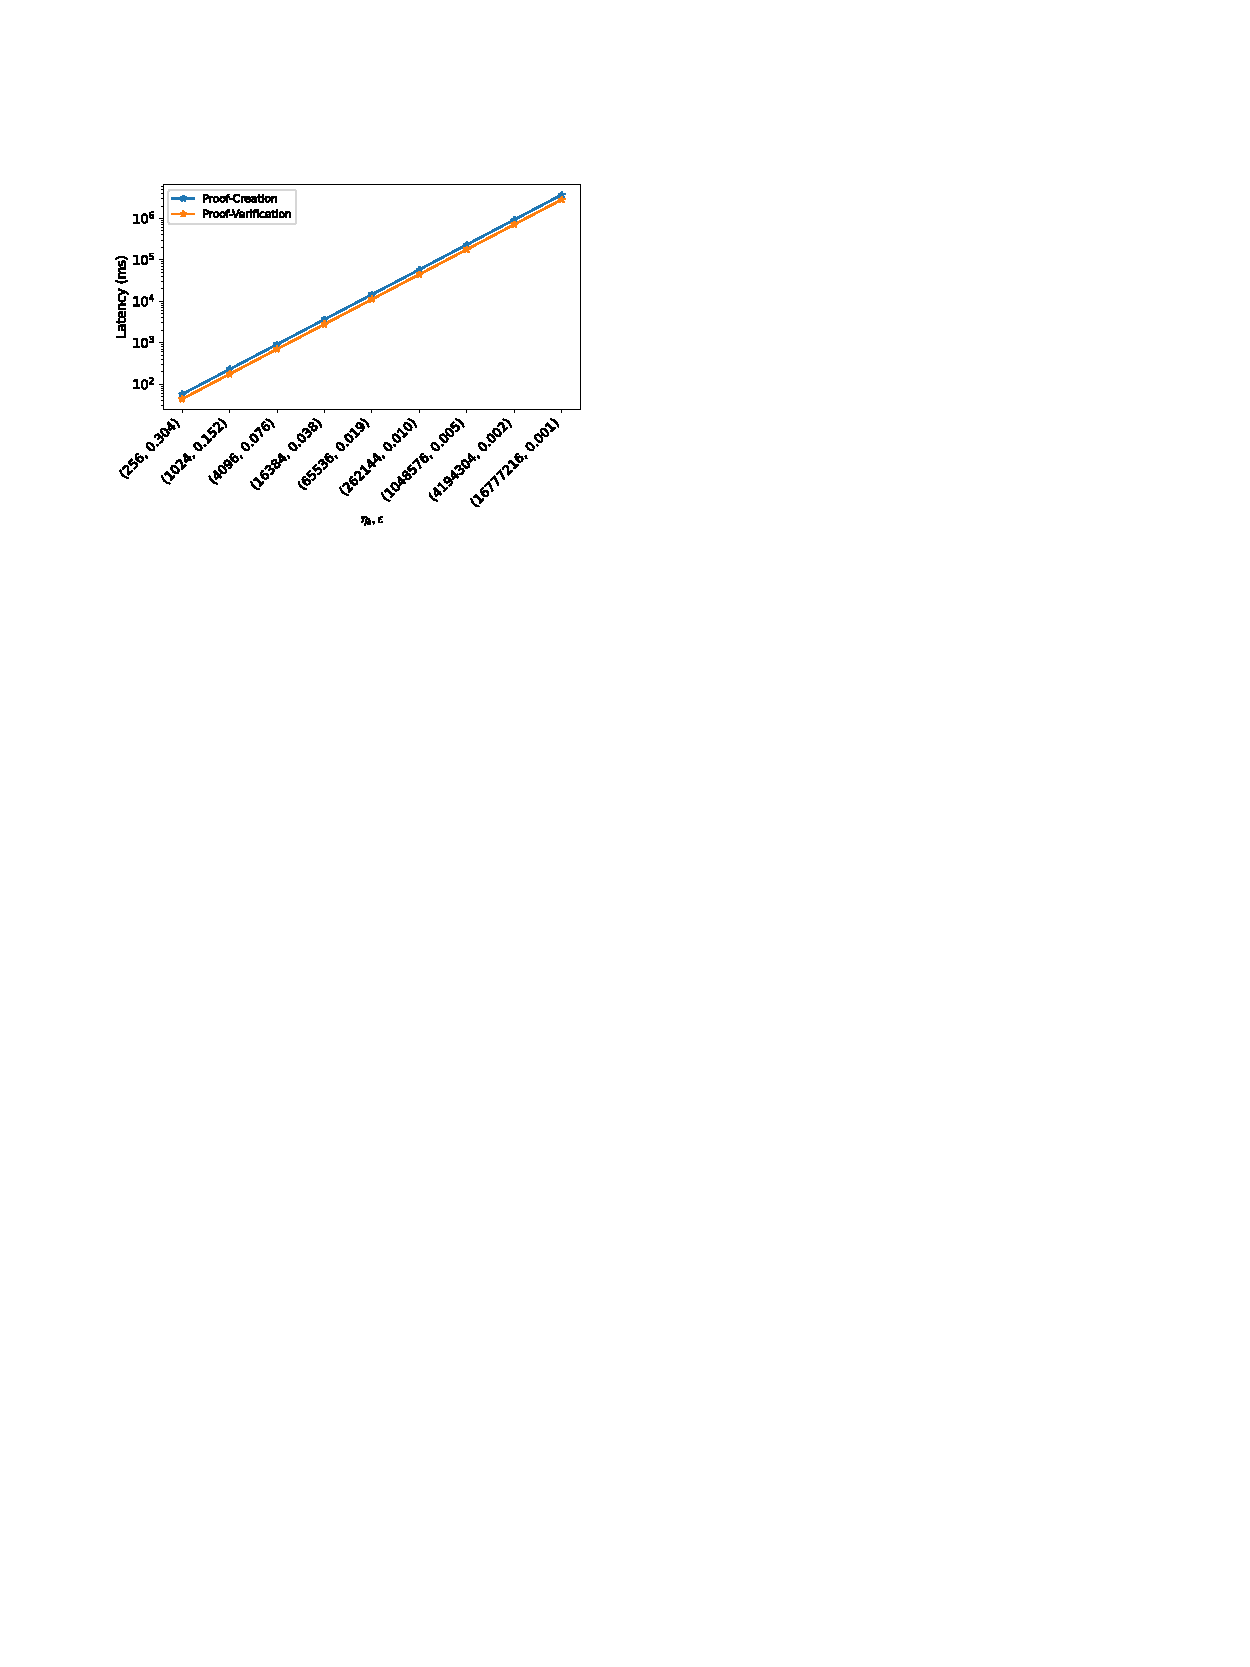
\includegraphics[scale=0.85]{pngs/eps_vs_coins.pdf}
     \caption{The figure above describes the latency of $\Sigma$-proof creation and verification as a function of the privacy parameters $\noisen$ and $\epsilon$. For a fixed $\delta=10^{-10}$, $\epsilon$ and $\noisen$ have one to one correspondence given by Lemma $\ref{theorem:dp_guarantee}$.}
     \label{fig:esp_vs_coins}
 \end{figure}


\paragraph{Time cost for client verification (MPC case)}
Clients submit secret shares of their inputs in the MPC setting. Thus the servers must verify that the client inputs are valid. For $M$-dimensional DP-histogram estimation, the client inputs are restricted to one-hot encoded vectors of size $M$. As discussed in Section \ref{sec:client_verification}, the sketching techniques used in PRIO and Poplar allow servers to verify clients with information-theoretic security. Still, they are vulnerable to attacks by malicious servers. Our use of $\Sigma$-OR-protocols can defend against such attacks, but it comes at a higher computational cost due to its reliance on commitments (which assume one-way functions exist). 
Figure~\ref{fig:client_verification} benchmarks the increase in latency as a function of the number of dimensions ($M$) of client input. We remark that the numbers in Figure \ref{fig:client_verification} are pessimistic as the Sigma-OR proof can be parallelised across the $M$ dimensions (at the cost of communication complexity), whereas the sketching techniques cannot as they are based on the inner products.
 \begin{figure}[t]
     \centering    
     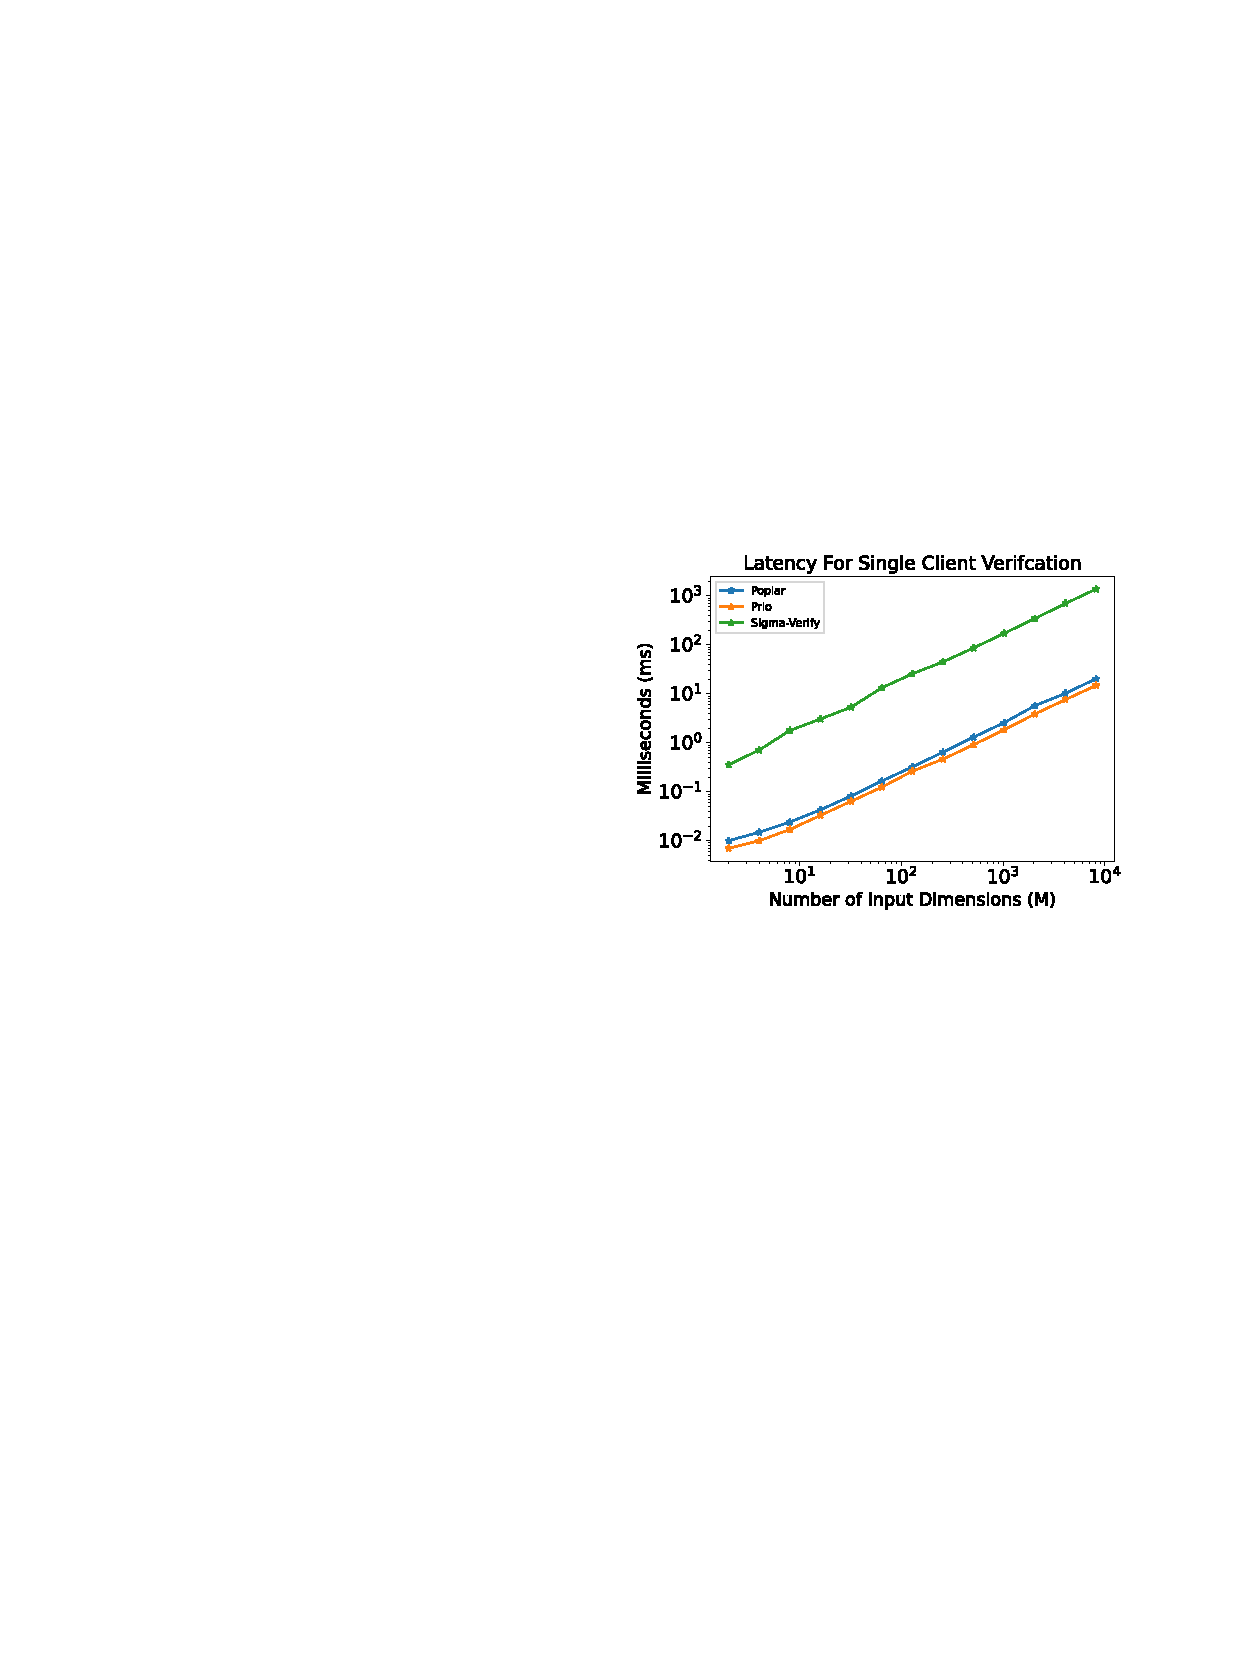
\includegraphics[scale=0.9]{pngs/verification_times.pdf}
     \caption{The figure above describes the performance cost for using a Sigma protocol to verify that the client's commitment is wellformed. PRIO and Poplar use lightweight sketching protocols and general-purpose MPC to check in zero knowledge whether a client's input is a one-hot vector and do not need to assume one-way functions exist. But as described earlier, they are susceptible to collusion attacks.}
     \label{fig:client_verification}
 \end{figure}


\section{Related Work}
\label{sec:related_work}
\UseRawInputEncoding

% Please add the following required packages to your document preamble:

\begin{table*}[]
\centering
\caption{Summary of efforts MPC computation of aggregate DP statistics. 
The active security column describes if the protocols allowed participants to deviate arbitrarily. The Central DP column describes if the protocol output satisfies constant DP error independent of the number of clients participating in the protocol. The auditable property describes if the final output can be verified for correctness. Some interactive protocols leak additional information (such as prefix information about client input bits) beyond just the DP output. The leakage column describes if the prescribed protocols suffered from additional leakage.}
\label{table:related_work}
\begin{tabular}{@{}lllll@{}}
\toprule
Protocol                                   & Active Security                                            & Central DP                        & Auditable                         & Zero Leakage                           \\ \midrule
\multicolumn{1}{|l|}{Cryptographic RR \cite{ambainis2004cryptographic}}  & \multicolumn{1}{c|}{$\checkmark$}                &  \multicolumn{1}{l|}{} &   \multicolumn{1}{c|}{}   & \multicolumn{1}{c|}{$\checkmark$}     \\
\multicolumn{1}{|l|}{Verifiable Randomization Mechanism \cite{kato2021preventing}}  & \multicolumn{1}{c|}{$\checkmark$}                &  \multicolumn{1}{l|}{} &   \multicolumn{1}{c|}{$\checkmark$}   & \multicolumn{1}{c|}{$\checkmark$}     \\
\multicolumn{1}{|l|}{Securely Sampling Biased Coins \cite{champion2019securely}}              & \multicolumn{1}{l|}{}                & \multicolumn{1}{c|}{$\checkmark$} & \multicolumn{1}{l|}{$\xmark$}     & \multicolumn{1}{c|}{$\checkmark$}     \\
\multicolumn{1}{|l|}{MPC-DP heavy hitters\cite{bohler2021secure}}              & \multicolumn{1}{l|}{}                & \multicolumn{1}{c|}{$\checkmark$} & \multicolumn{1}{l|}{$\xmark$}     & \multicolumn{1}{c|}{$\checkmark$}     \\
% \multicolumn{1}{|l|}{MPC-DP median \cite{bohler2020secure}}              & \multicolumn{1}{l|}{}                & \multicolumn{1}{c|}{$\checkmark$} & \multicolumn{1}{l|}{$\xmark$}     & \multicolumn{1}{c|}{$\checkmark$}     \\
\multicolumn{1}{|l|}{PRIO \cite{corrigan-gibbs_prio_2017}}              & \multicolumn{1}{l|}{}                & \multicolumn{1}{c|}{$\checkmark$} & \multicolumn{1}{l|}{$\xmark$}     & \multicolumn{1}{c|}{$\checkmark$}     \\
\multicolumn{1}{|l|}{Brave STAR \cite{davidson2021star}}        & \multicolumn{1}{l|}{}                 & \multicolumn{1}{l|}{}             & \multicolumn{1}{l|}{$\xmark$}     & \multicolumn{1}{l|}{} \\
\multicolumn{1}{|l|}{Sparse Histograms \cite{bell2020secure}} & \multicolumn{1}{l|}{}                 & \multicolumn{1}{c|}{$\checkmark$} & \multicolumn{1}{l|}{$\xmark$}     & \multicolumn{1}{l|}{} \\
\multicolumn{1}{|l|}{Crypt-$\epsilon$ \cite{roy2020crypt}}           & \multicolumn{1}{l|}{}                 & \multicolumn{1}{c|}{$\checkmark$} & \multicolumn{1}{l|}{$\xmark$}     & \multicolumn{1}{l|}{}             \\
\multicolumn{1}{|l|}{Poplar \cite{boneh_lightweight_2022}}            & \multicolumn{1}{c|}{$\checkmark$} & \multicolumn{1}{c|}{$\checkmark$} & \multicolumn{1}{l|}{$\xmark$}     & \multicolumn{1}{l|}{} \\
\multicolumn{1}{|l|}{Our work}          & \multicolumn{1}{c|}{$\checkmark$}                     & \multicolumn{1}{c|}{$\checkmark$} & \multicolumn{1}{c|}{$\checkmark$} & \multicolumn{1}{c|}{$\checkmark$}     \\ \bottomrule
\end{tabular}
\end{table*}

Dwork \etal introduced DP and described the Laplace mechanism for outputting histograms in the trusted curator model~\cite{dwork2006calibrating}.  Soon after, McSherry \etal proposed the exponential mechanism \cite{mcsherry2007mechanism} (equivalently, report noisy max \cite{ding2021permute}), which lets us compute the (approximately) most frequent bucket in a histogram, also under pure differential privacy.  Although these mechanisms give us pure differential privacy and optimal error rates $O(\frac{1}{\epsilon})$, implementing such a ``central'' model requires trusting that the curator to follow the protocol and not exploit the client data that it sees in plaintext. 


Therefore, researchers studied local privacy (LDP)  \cite{kasiviswanathan2011can} using randomised response \cite{warner1965randomized} to prevent any other party from seeing data in plaintext. 
Cheu, Smith and Ullman showed that the randomised response algorithm generalises all locally private protocols \cite{cheu2021manipulation}. 
This generalisation highlights two unavoidable disadvantages of local differential privacy. 
The first is that the accuracy of the protocol for even the binary histogram is $O(\sqrt{n})$ compared to $O(1)$ in the central model. 
The second is that randomised response systems offer a much weaker definition of privacy than the usual cryptography standards such as semantic security. 
For example, if the client flips their original answer with probability $p=0.1$, the curator sees their sensitive information in plain text 90\% of the time. 
Further increasing $p$ reduces the accuracy of the protocol dramatically. 
Consider the example from~\cite{corrigan-gibbs_prio_2017}, where 1\% of a million people answer ``yes'' to a survey about a sensitive topic. 
If we set $p=0.49$, then one-third of the time the central analyser concludes that not a single  member of the population answered ``yes''. 
Thus if we want to preserve utility, this definition of security is considerably weaker than the indistinguishability guarantees provided by protocols such as secret sharing.

Shuffle privacy \cite{cheu2021differential, balle2019privacy, erlingsson_amplification_2020} analyses local mechanisms under the lens of central privacy and bridges the accuracy gap between local and central models. 
Various results~\cite{ghazi_power_2020, balcer_separating_2020} prove that near central error guarantees are possible with distributed local transformations. Although this bypasses the accuracy issue of LDP, shuffle privacy assumes the existence of a secure shuffler, which is non-trivial to implement. 
Meanwhile, Bell \etal show that secure aggregation realises secure shuffling \cite{bell2020secure}. 
However, such protocols impose the impractical constraint of secure peer-to-peer communication between clients, and the curator is still a single source of failure. 
Despite the immense progress on differentially private histogram estimation, all known efficient implementations assume semi-honest participants and are a variant of either randomised response or the additive mechanism (where,  
additive mechanisms involve adding carefully curated randomness to the statistic before being released as output). 
It only takes a small fraction of clients to deviate from their prescribed protocol to destroy any utility of randomised response \cite{cheu2021manipulation}. 

% It is easy to see how byzantine participants could violate the utility and privacy of additive mechanisms. 
% For example, in the case of central privacy, the trusted server could simply output any value of their choice instead of following the protocol. 
% Or, the central server could reveal the randomness to an adversary $\AdvA$, who is then able to subtract randomness from the output.  
% The crux of the problem is that the participating clients do not have the means to validate the server's actions while receiving low error private aggregate statistics. 


To ensure central DP error without a trusted curator, Dwork \etal proposed using standard MPC for computing DP statistics~\cite{dwork2006our}. 
They proposed that each of the $K$ servers would own a fraction of the entire dataset used for computation. 
As long as not more than $\lfloor \frac{K}{3} \rfloor$ of the servers are dishonest, it is possible to compute DP-histograms with optimal accuracy. 
However, the protocol is not publicly auditable and breaks down in presence of a dishonest majority of adversarial corruptions. McGregor \etal show a separation between DP obtained using a trusted curator and that obtained using MPC \cite{mcgregor2010limits}. Specifically, they show that there exist computations (such as inner product or Hamming distance) where mechanisms with $(1, 0)$-DP incur $\Omega(\sqrt{n})$ reconstruction error compared to $O(1)$ in presence of a trusted curator. 
To bridge this gap, Mironov \etal defined computational differential privacy, a relaxation of traditional DP~\cite{mironov2009computational}. They show that as long as semi-honest OT exists, it is possible to compute any computationally DP function with the same error rates as information theoretic DP in a trusted curator model. 
Histograms, unlike inner product and Hamming distance, can be computed using MPC with the same error rates as trusted curator DP, under infomation theoretic DP. 
Thus recent work has focused on computing histograms using MPC. 

Bohler \etal use MPC to compute heavy hitters with semi-honest adversaries~\cite{bohler2021secure}. 
Researchers at Brave use oblivious pseudorandom functions (OPRF's) \cite{jarecki2009efficient} and Shamir secret sharing \cite{shamir1979share} to compute $k$-anonymous histograms in the two server setting~\cite{davidson2021star}.  However, they do not include support for differential privacy. Researchers at Google use linear homomorphic encryption and OPRFs to compute differentially private sparse histograms in two-server models (2PC)~\cite{bell2022distributed}, but require both the servers and clients to be semi-honest.
Corrigan-Gibbs propose PRIO, a protocol in which a small number of servers receive arithmetic shares of client input to compute differentially private histograms \cite{corrigan-gibbs_prio_2017}. PRIO uses shared non interactive proofs (SNIPs) to prevent clients from submitting illegal inputs but the protocol is only honest-verifier zero knowledge. Following the popularity of PRIO, Addanki \etal introduce PRIO+ to work over Boolean shares \cite{addanki2022prio+}. Boneh \etal use distributed point functions (DPFs) \cite{boyle2019secure} to compute DP heavy-hitters in the two server model to propose a system called Poplar \cite{boneh_lightweight_2022} that is zero knowledge even in presence of active adversaries. Roy \etal introduce \textit{Crypt}-$\epsilon$, a generic system to compute differentially private statisitcs using garbled circuits and linear homomorphic encryption \cite{roy2020crypt}. The general purpose natue of \textit{Crypt}-$\epsilon$ guarantees security only in the semi-honest threat model. Ambainis \etal proposed cryptographic randomised response \cite{ambainis2004cryptographic} but are able to only guarantee local differential privacy. Table \ref{table:related_work} summarises the assumptions under which the latest MPC protocols that have been used to compute DP statistics. As described earlier, existing work either assumes semi-honest adversaries or is not auditable. In 2021, the State Of Alabama sued the US deparment of commerce with regard to the errors caused due to random noise \cite{courtCase}. Differential Privacy by its defintion introduces a random noise blanket that tradesoff accuracy for privacy. This randomness is unavoidable if we wanted to protect individual privacy, but it also enables a corrupt aggregating server to disguise adversarial behaviour as randomness. In our paper, we first upgrade to security against active adversaries. Like existing literature we work in the dishonest majority model and further require the protocols to be publicly auditable. Our privacy constraints describe the most strict adversarial setting for practical deployment.

\section{Concluding Remarks}

We have introduced the notion of verifiable differential privacy to prevent malicious aggregators from using random noise as an attack vector. 
We have demonstrated the feasibility of this notion and showed that computational DP is necessary to achieve verifiability. 
A natural open question is to provide protocols for more complex DP mechanisms.  
Our protocol deliberately uses simple randomness (a Binomial distribution constructed from Bernoulli random variables), as making verifiable Laplace or Gaussian noise is far from clear.  
Similarly, approaches based on sampling from an appropriate distribution (the exponential mechanism) may be challenging since the distribution itself leaks information about the private data. 

\bibliographystyle{alpha-letters}
\bibliography{references}

\appendix

\input{Appendix/appendix.tex}
\appendix


\begin{figure}
    \centering
\begin{pchstack}[boxed, space= 0.7\fboxsep]  % default 
    \pseudocode[linenumbering , skipfirstln]{%
    \textbf{Verifier} \< \< \textbf{Prover} \\[][\hline]
     \< \text{ Common Input } g, h, \G_q, q, c \<    \\[-5pt]
    \<\<b,  v_1, e_1 \xleftarrow{R} \Z_q; \\[-5pt]
    \<\<\text{Set } d_0 = h^b \text{ and } d_1 \text{ such that }d_1\Big(\frac{c}{g}\Big)^{e_1} = h^{v_1}\\[-9pt]    
    (d_0, d_1) \< \sendmessageleft*{(d_0, d_1)} \<(d_0, d_1) \\[-7pt]
    e \xleftarrow{R} \Z_q \< \sendmessageright*{e} \< e_0 = e - e_1 \mod q; v_0 = b + e_0r_x \\[-9pt]
    \text{Check } e_1 + e_0 = e \< \sendmessageleft*{(v_0, e_0, v_1, e_1)} \< \\[-9pt]
    \text{Check }d_0c^{e_0} = h^{v_0} \text{ and } d_1c^{e_1} = g^{e_1}h^{v_1}\<\<
}
\end{pchstack}    
    \caption{Proof for convincing $\Verifier$ that $c_x = g^xh^{r_x}$without revealing the value $x=0$.}
    \label{fig:schnorr_or_a}
\end{figure}


\begin{figure*}[!h]
    \centering
\begin{pchstack}[boxed]  % default  
    \pseudocode[linenumbering , skipfirstln]{%
    \textbf{Verifier} \< \< \textbf{Prover} \\[][\hline]
     \< \text{ Common Input } g, h, \G_q, q, c \<   \\[-5pt]
    \<\< b, v_0, e_0 \xleftarrow{R} \Z_q\\[-5pt]
    \<\<\text{Set } d_1 = h^b \text{ and }d_0 \text{ such that }d_0c^{e_0} = h^{v_0}\\[-9pt]    
    (d_0, d_1) \< \sendmessageleft*{(d_0, d_1)} \<(d_0, d_1) \\[-9pt]
    e \xleftarrow{R} \Z_q \< \sendmessageright*{e} \< e_1 = e - e_0 \mod q ; v_1 = b + e_1r_x\\[-9pt]
    \text{Check } e_1 + e_0 = e \< \sendmessageleft*{(v_0, e_0, v_1, e_1)} \< \\[-9pt]
    \text{Check }d_0c^{e_0} = h^{v_0} \text{ and } d_1c^{e_1} = g^{e_1}h^{v_1}\<\<
}
\end{pchstack}    
    \caption{Proof for convincing $\Verifier$ that $c_x = g^xh^{r_x}$without revealing the value $x=1$.}
    \label{fig:schnorr_or_b}
\end{figure*}


\section{Formal Security Definitions}
\label{app:sec_defns}

\begin{definition} [Discrete Log Assumption]Let $\SecurityParam$ denote the security parameter.
For all PPT adversaries $\AdvA$, there exists a negligible function $\Negl$ such that 
     \[ \Pr\left[ x = x^\prime : \begin{array}{c} \pp = (\G_q, g) \samples \texttt{Setup}(1^\kappa) \\
     x \samples \Z_q, h = g^x \\
       \AdvA(\pp, h) \outputs x^\prime \\
    \end{array} \right]
  \leq \mu(\kappa)  \] 

\label{defn:discrete_log}
\end{definition}

\begin{definition} (Hiding Commitments) Let $\SecurityParam$ be the security parameter. Let $\MessageSpace_\pp$ and $\RandomnessSpace_\pp$ denote the message space and randomness space of the commitment scheme as parameterised by public parameters. A commitment scheme is said to be \textit{hiding} for all PPT adversaries $\AdvA$, if the following quantity is negligible. The commitment is \textit{perfectly hiding} if $\Negl(\SecurityParam) = 0$.
\label{defn:hiding_com}
     \[ \Pr\left[ b = b^\prime : \begin{array}{c} \pp \samples \texttt{Setup}(1^\kappa) \\
     b \samples \bit, r_{x_b} \samples \RandomnessSpace_\pp \\
      \AdvA(\pp) \outputs (x_0, x_1) \in \MessageSpace_\pp\times \MessageSpace_\pp  \\
     c = \Com(x_b, r_{x_b}) \\
      \AdvA(\pp, c) \outputs b^\prime
    \end{array} \right]
  \leq \mu(\kappa)  \] 
\end{definition}

\begin{definition} (Binding Commitments) Let $\SecurityParam$ be the security parameter. Let $\MessageSpace_\pp$ and $\RandomnessSpace_\pp$ denote the message space and randomness space of the commitment scheme as parameterised by public parameters. A commitment scheme is said to be \textit{binding} if, for all PPT adversaries $\AdvA$, there exists a negligible function $\Negl$ such that

\label{defn:binding_com}
     \[  \Pr\left[ \Com(x_0, r_0)= \Com(x_1, r_1) \land x_0 \neq x_1 : \begin{array}{c} \pp \samples \texttt{Setup}(1^\kappa) \\
       \AdvA(\pp) \outputs x_0, r_{x_0}, x_1, r_{x_1}  \\     
    \end{array} \right]
 \leq \frac{1}{2} + \mu(\kappa)  \] 
The commitment is \textit{perfectly binding} if $\mu(\kappa) = 0$.
\end{definition}

% \input{Appendix/b_dp_proofs}
%\input{Appendix/c_fiat_shamir}


\section{OR Protocol}
\label{app:sigma_open}
\ariInline{Needs work}

Define as public parameters a cyclic prime order group $\G_q$ and generators $g$ and $h$ for $\G_q$. 
Let $\mathcal{M}_\pp = \mathcal{R}_\pp = \Z_q$. 
Pedersen Commitments defined in~\eqref{eq:pedersen} satisfy all properties described in Section~\ref{sec: commitments}.
%
\begin{equation}
    \Com(x, r_x) = g^xh^{r_x}
    \label{eq:pedersen}
\end{equation}

For the sake of completeness, we describe the interactive disjunctive OR proof using $\Sigma$-protocols from \cite{cramer1994proofs}. Note that the $\Sigma$ protocols are cheating verifier zero knowledge even without a random oracle. Maurer \cite{maurer2009unifying} shows that if the verifier's challenge space is polynomial sized, then the protocol can be shown to be zero knowledge. Damgard \etal show that by using Trapdoor commitments \cite{damgaard2000efficient}, one can preserve soundness and get zero knowledge but the protocol now has four messaging rounds instead of 3. Next, we describe the $\Sigma$-protocol that can be used to verify the OR condition. \par 
Let $x \in \bit$ and $c_x = \Com(x, r_x)$ for $r_x \samples \Z_q$ be the commitment to $x$. 
Given $c_x$, $\OrProtocol$ is an interactive zero knowledge proof between a prover $\Prover$ and a PPT verifier $\Verifier$ to show that $c_x \in \BitLang$. 
The security properties can be found in \cite{thaler2020proofs, damgaard2000efficient, cramer1994proofs}.  Figure~\ref{fig:schnorr_or_a} and Figure~\ref{fig:schnorr_or_b}  succintly describe the OR protocol to prove that for some $r_x \in \Z_q$, $c_x \in \BitLang$. 
%
\begin{equation}
\BitLang = \{c_x: x \in \bit \land c_x = \Com(x, r_x) \}    
\end{equation}

Based on the value for $x$, the prover uses the protocol described in . The verifier cannot distinguish between the protocol's two runs as the messages are indistinguishable. In case the the inputs $\vec{x}$ are bit strings of size $M$ (like in PRIO and Poplar) and only one coordinate can be non-negative, the prover sends to the verifier $r = \sum_{j=1}^M r_{x_j}$ along with the $\Sigma$-proofs, where $r_{x_j}$ is the randomness used to create commitments for the coordinate $x_j \in \bit$. As $\vec{x} \in L$, implies $\vec{x} \in \bit^M$ and $|| \vec{x}||_1 = 1$, the OR proofs verify the first criterion and the second criterion is easily verified by checking $c_{|| \vec{x}||} = \prod_{j=1}^M c_{x_m}$ is a a commitment to one i.e., check if $g^1h^r = c$. 


\section{Deferred Security Proofs}
\label{app:single_curator_sec_proof}

\paragraph{Single Curator Simulator Proof}
\ariInline{Needs the right theorem numbering}

\stateboxsolid{
\begin{thm}
Let  $\ChVerifier$ denote the corrupted verifier. There exists a PPT Simulator $\Simulator^{\ChVerifier}$ such that for if $y \samples \Mechanism_\bin(X, Q)$, then

 \begin{align*}
    \View\left[\Pi(\Prover, \ChVerifier_{[z]})\right] &\stackrel{c}{\equiv} \Simulator^{\ChVerifier}(y, \vec{r}_\Verifier, z, \pp)        
    \end{align*}

    where $z \in \bit^{\poly(\SecurityParam)}$ and $\vec{r}_v \in \bit^{\poly(\SecurityParam)}$ represents auxiliary input and randomness available to all the corrupted parties.  	
\end{thm}
}


\begin{proof}
Denote the corrupted verifier as $\ChVerifier$.  $\Simulator$ receives on its input tape the inputs for $\ChVerifier$. The ideal oracle functionality $\Mechanism_\bin$ is defined as before. Let $\Simulator$ denote shorthand for $\Simulator^{\ChVerifier}$. 
We construct the simulator as follows:
\begin{enumerate}    
    \item{$\Simulator$ receives the public messages $\{c_i\}_{i \in [n]}$.}
%
    \item{$\Simulator$ invokes $\Mechanism_\bin$ with the empty string $\lambda$ and receives $y$ as defined in equation \eqref{eq:M_bin}.
    }
%    
    \item{$\Simulator$ samples $z \samples \RandomnessSpace_\pp$ and sets $c = \Com(y, z)$.}

    \item{$\Simulator$ samples $c'_{2}, \dots, c'_{{\noisen}}$ such that $c'_{j} = \Com(1, s_{j})$ where $s_{j} \xleftarrow[]{R} \mathcal{R}_\pp$. It sets $c'_{1} = g^1a$ where $a = c \times  \Big( \prod_{j=2}^{\noisen} \hat{c}'_{j}\Big)^{-1} \times \Big( \prod_{i=1}^{n} c_{i}\Big)^{-1} \times g^{-1}$.
     }
%    
     \item{$\Simulator$ sends over $\{c_{j}\}_{j \in [\noisen]}$ to $\AdvA$ pretending to be the honest prover (Line 4 of Figure \ref{fig:dp_interactive_proof}).
     }
	    
    \item{$\Simulator$ pretends to be the prover and jointly invokes $\oracle_{\Morra}$ with $\AdvA$ to sample $\noisen$ unbiased public bits $(b_{1}, \dots, b_{\noisen})$.}
%    
    \item{$\Simulator$ sends $y$ and $z$ to $\AdvA$ and outputs whatever $\AdvA$ outputs.}
\end{enumerate}
\end{proof}
%\endinput
%

\end{document}
